\chapter{Biomedical text classification and similarity measurement}
\label{c4}

Text classification or categorization can represent a different number of tasks.
The most primitive one is to simply identify if a given text is relevant or not according to some criteria---that is, for example, if a news article is about a specific subject or a clinical record contains valuable information about a specific disease.
This is known as binary text classification since there are only two possible outcomes---\textit{yes} or \textit{no}.
On the other hand, in multi-class classification there are several, three or more, possible classes and only a single one must be chosen.
Another problem is multi-label classification where none, one, or more topics (classes) can be associated with a document.

The \as{nlp} task of sentiment analysis is an example of text categorization where different emotion states can be associated with a fragment of text often collected from social media \parencite{feldman2013a,liu2015d,bouazizi2016a,tao2020a}.
Another common application of text classification is spam filtering in eletronic mail (\as{email}) systems where unsolicited \as{email} messages should be detected and discarded \parencite{diao2000a,zhang2004a,bhowmick2018a}.

Document triage, document filtering, or document selection is a text classification task that can be employed to select the most relevant documents for a specific information extraction task.
Although \textcite{hearst1999a} argues that categorizing documents does not lead to discovering new information, \textcite{sarawagi2008a} explains that document classification is relevant (for information extraction) as a first step to filter out less-relevant documents especially if the corpus is very large.
Similarly, \textcite{balog2018a} clarifies how the task of scoring documents according to how relevant they are to a given target entity is helpful for information extraction.

Text classification can be thought as grouping and clustering texts that share some degree of similarity concerning some aspect.
For instance, if a text is considered to be relevant regarding a specific criterion then it is likely that similar texts may also be of interest.
For that reason, we consider that measuring the semantic textual similarity is a intertwined task with text classification.
Therefore, in this chapter, we also review and present work on text similarity measurement despite being applicable in distinct \as{nlp} tasks such as word sense disambiguation and relation extraction.

Measuring the semantic similarity between texts is the basis of many text processing tasks.
For example, finding excerpts of text with redundant information can be used for summarization \parencite{aliguliyev2009a}.
Another use case is plagiarism detection where texts with equivalent semantics are identified \parencite{lukashenko2007a}.
Semantic similarity measurement can also be used to find similar textual contexts in which a relationship holds between specific entities \parencite{panchenko2012a}---if two concepts have a certain interaction and two other different concepts appear surrounded by a similar textual context then it is likely they have a similar or the same interaction.

This chapter addresses two analogous \as{nlp} tasks: (1) text classification and (2)~measurement of semantic textual similarity.
We start by giving a brief overview of these problems applied in the biomedical domain and then present our solutions.
First, a study with supervised machine learning classifiers is conducted for scientific literature triage.
Then, a hybrid system based on rules and machine learning for categorizing clinical text is presented.
Finally, a neural network that quantifies the textual similarity between clinical sentences is presented.


\section{Background}

The problem of \textit{text classification} or \textit{text categorization} is likely one of the oldest and most addressed tasks of natural language processing and has been relevant for many years in information retrieval \parencite{lewis1995a,manning2008a}.
Early work on text categorization was focused on selecting different features from syntactic analysis \parencite{lewis1992a}, where the simplest approach would be to treat each word as a feature.
Later, \textcite{joachims1998a} proposed the use of support vector machines for text categorization and argued these are robust models because they eliminate the need for feature selection, show good performance, and do not require manual parameter tuning.

In the biomedical domain, to the best of our knowledge, \textcite{craven1999a} was one of the pioneer works employing text classification methods to identify relevant textual information, from 2889~abstracts in the \as{medline} database, for constructing biomedical knowledge bases.

\textcite{feldman2003a} review past work on text mining of the biomedical literature.
Particularly, the authors emphasize the importance of text categorization as an early step of pre-processing since reducing the set of documents simplifies the follow-up mining tasks such as entity and relation extraction.
Furthermore, they explain that there are two main approaches for text categorization: (1) the \textit{knowledge engineering} approach where expert knowledge is manually encoded using a set of rules, and (2) the \textit{machine learning} approach where a text classifier is built automatically by learning from a set of previously classified documents using a pre-defined set of categories.
They also distinguish two main methods in the machine learning approach: in one method, for each pair of document and category, a boolean value is attributed---true if the document belongs to the category or false otherwise; in the other method, a value between~0 and~1 representing the confidence that the document belongs to the category is assigned, and afterwards document are ranked according to their confidence value.

\textcite{cohen2005a} also present an extensive review of past work on biomedical text mining and text classification.
The authors argue that text classification systems are valuable to biomedical database curators because they may have to review some documents until finding a particular piece of information for updating the database.
\textcite{yeh2003a} conducted a text mining competition in the \as{kdd} (Knowledge Discovery and Data Mining) Challenge Cup\footnote{\url{https://kdd.org/kdd-cup/view/kdd-cup-2002/Tasks}} aimed at identifying which biomedical articles were relevant for curating \textit{Drosophila} gene expression information.
The organizers provided a training set of 862~journal articles curated in FlyBase \parencite{theflybase2002a} with genes and gene products, and a test set with 213~new articles.
Participating teams had to develop a system that indicated which articles contained experimental evidence for gene expression products.
The best performing team \parencite{regev2003a}---that obtained 78\%~F-measure in the document curation sub-task---manually built text rules for matching common patterns in the title, abstract, and figure captions, and performed part-of-speech tagging and text chunking.
In a different work, \textcite{donaldson2003a} used a support vector machine to find protein--protein interaction data on the \as{pubmed} literature database and estimated that their system spared curators several days of work because they had to scan a significantly lower number of abstracts.
The \as{trec} (Text Retrieval Conference) 2004 Genomics Track \parencite{voorhees2004a,hersh2004b,hersh2005a} addressed a triage task of full-text documents, simulating the work of curators in the Mouse Genome Informatics (\as{mgi}) system, where participants had to develop automatic solutions for detecting articles containing experimental evidence requiring the assignment of Gene Ontology (\as{go}) codes.

The Computational Medicine Center in Cincinnati, Ohio organized a shared task to promote the development of automatic systems for assigning \as{icd}-9-CM\footnote{International Classification of Diseases, Ninth Revision, Clinical Modification. \url{https://www.cdc.gov/nchs/icd/icd9cm.htm}} codes to radiology reports \parencite{pestian2007a}.
The challenge corpus was annotated by coding staff of CCHMC (Cincinnati Children's Hospital Medical Center) and two independent coding companies in order to reduce variation due to human judgment.
It was split into training and testing sets with~978 and 976~documents respectively, and tagged with forty-five \as{icd}-9-CM distinct labels.
This multi-label classification task allowed each record to be assigned more than one code.
The participating team from the University of Pennsylvania \parencite{crammer2007a} employed a cascaded approach combining three coding systems: (1)~a specialized policy that searched for specific keywords complying with some heuristics, (2)~a rule-based system that checked if \as{icd}-9-CM code descriptions appear in the reports, and (3)~a learning system that used several natural language features.
They achieved a micro-averaged F1-score of 0.8760 on the test set ranking 4th out of 44 systems that entered the challenge.
Another team, from the University of Manchester \parencite{sasaki2007a}, employed different machine learning algorithms and tested different features such as n-grams of words weighted by \as{tf}--\as{idf} values.
They ranked 5th in the challenge and their best result, a micro-averaged F1-score of 0.8594 on the test set, was achieved by a support vector machine.
In another work, \textcite{farkas2008a} investigated the feasibility of automatically constructing rule sets---in contrast to purely handcrafted rule-based systems---by replacing several laborious steps with machine learning models with the aim to alleviate the manual work from experts.
Their system achieved competitive results with a micro-averaged F1-score of 0.8893 on the test set, and the authors concluded that hybrid systems preserve the good performance of rule-based classifiers and that, with the help of machine learning methods, their construction can be accelerated and require less human effort.
More recent works explore the use of deep neural networks for automatic \as{icd}-9 coding in clinical reports \parencite{pereira2018c,zeng2019b}.

Other international challenges on biomedical text classification have been conducted in recent years to encourage the creation of text mining solutions and assess the state-of-the-art.
We close this brief roadmap by presenting three competitions offered by the BioCreative organizers but we alert the reader that additional research work, not mentioned here, has been carried out \parencite{huang2016a}.
In the BioCreative~III \as{ppi} ACT (article classification task) participants had to implement systems for detecting \as{pubmed} abstracts describing protein--protein interactions \parencite{krallinger2010a,krallinger2011a}.
The organizers prepared a dataset split into training, development, and test partitions with 2280, 4000, and 6000 abstracts respectively which were manually labeled by domain experts.
BioCreative~VI launched a document triage task for precision medicine where the aim, for participating systems, was to identify \as{pubmed} abstracts describing genetic mutations affecting protein-protein interactions---our contribution on this problem is presented in \Cref{c4:s:literature-triage}.
In BioCreative~VII, \textcite{chen2021b,chen2022c} promoted a challenge on \as{covid19} literature curation since the number of \as{covid19} related articles was growing at a rate about 10\,000 articles per month.
Their effort tackled a multi-label topic classification for \as{covid19} literature to alleviate the burden of manual topic annotation in the LitCovid database \parencite{chen2021c} which contained tens of thousands of \as{pubmed} articles relevant to \as{covid19} that needed to be assigned with up to eight distinct topics (such as \textit{case report}, \textit{diagnosis}, and \textit{treatment}).

To the best of our knowledge, a great part of the research work on the task of measuring the semantic textual similarity (\as{sts}) has been performed for the general-domain and originated from the \as{semeval} \as{sts} task series \parencite{agirre2012a,agirre2013a,agirre2014b,agirre2015a,agirre2016a}.
On the other hand, regarding \as{sts} between biomedical text snippets there has been less investigation and only a few manually annotated datasets have been made available \parencite{sogancioglu2017a,wang2018d,wang2020d}.
\textcite{wang2018e,wang2020d} organized the first shared tasks on clinical \as{sts}
and captured the attention of many research teams around the world that proposed their systems---our contribution on this problem is presented in \Cref{c4:s:clinical-sts}.
For example, \textcite{chen2021a} benchmarked several top-ranked deep learning models for measuring the relatedness between sentence pairs in the clinical domain.
They evaluated word embedding--based models such as convolutional neural networks, sentence embedding--based models such as the BioSentVec pre-trained model \parencite{chen2019g}, and transformer-based models such as BioBERT \parencite{lee2020a}, BlueBERT \parencite{peng2019a}, and ClinicalBERT \parencite{alsentzer2019a}.
The authors concluded that BioSentVec and BioBERT achieved the highest results but emphasize that BERT models are much slower than the convolutional neural network and BioSentVec models.

Lastly, for further reading, we point the reader to other survey works on text classification \parencite{aggarwal2012a,mironczuk2018a,altinel2018a,kowsari2019a,minaee2022a} and similarity measurement \parencite{wang2020c,chandrasekaran2021a}.


\section{Literature triage for precision medicine}
\label{c4:s:literature-triage}

Identifying relevant literature for harvesting particular biomedical knowledge is a paramount task, but expert curators invest a significant amount of time manually performing this annotation \parencite{fang2012a,karp2016a}.
There are scientific articles that are more pertinent for extracting specific biomedical information such as protein--protein interactions or adverse drugs effects; and thus, the development of automatic solutions for biomedical document triage is essential and helpful to alleviate the manual annotation work by professional curators.
Also, a reduced number of more appropriate candidate documents allows automatic \as{ie} systems to take more time for making their predictions---regarding biomedical named entities and their relations---with a superior performance, and therefore a document classification step is crucial for eliminating noisy or less-relevant documents.

In this section we present supervised machine learning models for selecting biomedical documents relevant for precision medicine.
The aim of precision medicine is to select the best treatments for different patient groups, considering individual variability in genes, environment, and lifestyle.
Regarding genetic variability, valuable information about variants and how they affect protein--protein interactions is available in the scientific literature.
Extracting and curating this information in an efficient manner requires the application of text mining algorithms.
In this work, we experimented with classical machine learning and neural network classifiers for predicting which \as{pubmed} abstracts contained relevant information for extracting protein--protein interactions (\asp{ppi}) affected by genetic mutations.
We also evaluated the impact of including additional training data from a similar dataset, containing general \asp{ppi}, as a semi-supervised or self-training approach.

The Precision Medicine task, part of the BioCreative~VI community challenge in biomedical text mining, aimed to evaluate text mining approaches and tools for identifying and extracting information regarding the impact of genetic mutations on protein--protein interactions \parencite{dogan2017a,dogan2019a}.
The challenge consisted of two subtasks, namely document triage and relation extraction.

The application of text mining and automatic classification tools for document triage was evaluated in the BioCreative~III \as{ppi} article classification task where the aim was to classify and rank articles relevant for curating protein--protein interactions \parencite{krallinger2010a,krallinger2011a}.
The best system was based on a large margin classifier with features derived from gene named entity recognition, MeSH terms, and dependency parsing, and reached an area under the interpolated Precision/Recall curve (\as{auc} iP/R) of 0.6798 and an F1-score of 0.6142 \parencite{kim2011e,kim2011d}.


\subsection{Materials and methods}

We followed a supervised machine learning approach, and evaluated classical classifiers against deep learning models.
In both cases, we used word embeddings to represent the words in the documents.


\subsubsection{Data}

The Precision Medicine task organizers provided a dataset split into training and test subsets consisting of 4082 and 1427~\as{pubmed} abstracts respectively, which were manually classified as relevant, that is, containing information regarding the impact of gene mutations on protein--protein interactions, or not relevant.
\Cref{tab:pm-dataset} presents the statistics of the Precision Medicine track dataset in detail.

\begingroup

\begin{table}[!tb]

\caption{Statistics of the Precision Medicine track dataset.}
\label{tab:pm-dataset}

\centering

% \small

\begin{tabular}{D{30mm}G{20mm}G{20mm}G{20mm}}

\toprule

Partition & Abstracts & Positive & Negative\\

\midrule

Training  & 4082 & 1729 & 2353\\
Test      & 1427 &  704 &  723\\

\midrule

Total     & 5509 & 2433 & 3076\\

\bottomrule

\end{tabular}
\end{table}
\endgroup


Apart from this annotated dataset, we exploited the use of the BioCreative~III PPI ACT corpus as additional data \parencite{krallinger2010a,krallinger2011a}.
This corpus consists of 12\,280 \as{medline} abstracts, 2732 of which were annotated as containing PPI information.
Although this annotation does not consider the impact of genetic mutations, as is the case of the task considered here, we tried to incorporate this data in a self-training approach.


\subsubsection{Word embeddings}

We used the word2vec implementation in the Gensim framework \parencite{rehurek2010a} and generated word embeddings from the complete \as{medline} database, corresponding to 15 million abstracts in English language.
We created six models with vector sizes of 100 and 300 features and windows of 5, 20, and 50.
The models contain around 775 thousand distinct words.
We conducted several preliminary experiments using cross-validation on training data with these six variants of word embedding models, and our results demonstrated that the word embeddings model with 300 features and window size of 50 provided the best result for almost every configuration.
Therefore, in this work, all the classifiers tested and presented here used the model with 300 features and window size of 50.


\subsubsection{Classical classifiers}

We compared three classifiers from the scikit-learn library \parencite{pedregosa2011a}: k-nearest neighbors (\as{knn}), logistic regression (\as{lr}), and multi-layer perceptron (\as{mlp}).
For the sake of readability, we denote these as \textit{classical} classifiers because they are commonly employed in text classification and their off-the-shelf implementations, offered by scikit-learn, can be applied straightforward to this task with little effort.
We used the default hyperparameters defined by scikit-learn with the exception of the following values: the \as{knn} used a number of neighbors of 99, and the \as{mlp} used a maximum of 2000 iterations for convergence.
These classifiers were favorably chosen because their implementation allows to predict probability estimates which was relevant for this task since the system had to return a confidence value for the prediction.
For example, if the system predicts that an article is relevant then it is also valuable to know how much confidence the system has in its prediction.
Also, these classifiers were selected because they provided solid results in previous research on document classification \parencite{kamath2018a,kadhim2019a,shah2020a}.

To obtain the document representation for the classifier, we tokenized the document and obtained the sequence of word vectors by simple look-up in the pre-calculated word2vec embeddings model.
However, these classifiers are not directly applicable to sequences of distinct length and some form of aggregating these sequences is required.
This is commonly addressed by summing or averaging the word vectors, resulting in a single vector representation of the document.
We followed a similar approach, a weighted average of the word vectors, where each word vector was weighted by its \as{tf}--\as{idf} value pre-calculated from the training data---note that for cross-validation evaluation the \as{idf} values were calculated for every subgroup containing only the training partitions.


\subsubsection{Deep learning classifiers}

We applied different deep learning strategies based on (1) convolutional and (2) long short term memory (\as{lstm}) layers.
Convolutional neural networks (\asp{cnn}) have been extensively applied in image recognition and classification problems with very good performance \parencite{rawat2017a}, and various works also demonstrate their application in text classification tasks \parencite{rios2015a}.
On the other hand, \as{lstm} networks which are a special type of recurrent neural networks (\asp{rnn}) can be more adequate for text-based tasks due to the sequential structure of natural language text, since these models contain feedback connections and can learn long-term dependencies in the input sequences \parencite{hochreiter1997a,graves2012b}.

Overfitting in the training data is a common problem when using deep neural networks since they have a strong pattern-memorization ability.
In general, the higher the number of layers and neurons they have the stronger their tendency to memorize and overfit.
For that reason, in our experiments we included different strategies---early stopping, dropout, and regularization---to avoid overfitting.

Our early stopping technique consisted in being vigilant of the loss value in a validation subset (for every training epoch) and terminating the training process if the loss did not decrease after five consecutive epochs.
We used 10\% of the training data, selected randomly, as validation set.
We applied dropout to the output of the embedding and hidden layers so that a random selection of the output tensors is not used for updating the model weights, with the aim of forcing the model to learn a less biased representation of the data.
Finally, L2 regularization is applied to the final layer to penalize large weights that could otherwise be assigned to biased input dimensions.

Differently from the classical classifiers that used a weighted average of the word vectors to represent each document, in the case of these deep neural network classifiers each document was represented by the concatenated sequence of its word vectors where a maximum sequence length of 1000~words was considered.
This document representation was then forwarded to a convolutional recurrent neural network.

We empirically tested various network architectures and built three different systems based on convolutional and \as{lstm} layers for the official evaluation in the task since, in comparison to the classical classifiers, these deep learning models provided superior results according to preliminary cross-validation experiments on training data (\Cref{tab:pm-cv-results}).
All models were trained using the binary cross-entropy loss function and the RMSProp algorithm as optimizer \parencite{hinton2012a}.
Models were implemented in the Keras framework \parencite{chollet2015a} with the TensorFlow backend \parencite{abadi2016a} and executed on a machine with 12~\as{cpu} cores and 192~GB of memory.


\paragraph{System 1}

The first system consists of a network architecture starting with an embedding layer, that represents each word in a document by its respective word vector, followed by three convolutional layers with average pooling.
Each convolutional layer uses 128 filters with \as{relu} (rectified linear unit) activation and a kernel size of 3.
The output is then connected to a bidirectional \as{lstm} layer with 128 units, and to a final densely connected layer with sigmoid activation and L2 regularization with a penalty factor of 0.01.
A dropout of 0.1 was included after the embedding layer and of 0.2 within the \as{lstm} units.

This model was trained using 90\% of the training data from the Precision Medicine dataset (10\% left for validation), with a batch size of~32 samples and for a maximum of 100~epochs.


\paragraph{System 2}

In the second system we followed a self-training approach to incorporate the BioCreative~III \as{ppi} corpus as additional data.
Since this corpus is annotated following different guidelines, we first applied the trained model from System~1 to infer the relevance of these documents and selected the ones that were classified with a confidence value higher than 0.90.
This equated to adding 9673 documents, all \textit{pseudo-labeled} as not relevant, to the training data.
The same network was then re-trained from scratch with the combined dataset, and a validation subset containing 10\% of the training data from the Precision Medicine dataset was used to monitor the model performance during training.


\paragraph{System 3}

The third system is similar to the System~1 but consists of a deeper network composed of three convolutional layers and three \as{lstm} layers.
The first layer of the network is the embedding layer as in Systems~1 and~2, but a dropout of 0.2 is applied to the embedding vectors.
This layer is followed by three convolutional layers with average pooling, and each convolutional layer uses 64 filters with \as{relu} activation and a kernel size of 5.
A dropout of~0.4 is applied after each pooling stage.
This is then followed by a bidirectional \as{lstm} layer and two unidirectional \as{lstm} layers.
All \as{lstm} layers are composed of 128 units and use a dropout of 0.2.
Finally, a dense layer is applied with sigmoid activation and L2 regularization with a penalty factor of 0.01.


\subsection{Results and discussion}

\begingroup
% \newcommand{\z}{\hphantom{0}}

\begin{table}[!tb]

\caption%
[Five-fold cross-validation results on the Precision Medicine training set with classical and deep learning classifiers.]%
{Five-fold cross-validation results on the Precision Medicine training set with classical and deep learning classifiers. The highest F1-score is highlighted in bold. k-NN: k-nearest neighbors. LR: logistic regression. MLP: multi-layer perceptron.}
\label{tab:pm-cv-results}

\centering

% \small
% \normalsize
% \large

\begin{tabular}{E{40mm}T{19mm}T{19mm}T{19mm}}

\toprule

& Precision & Recall & F1-score\\

\midrule

\multicolumn{4}{l}{\textit{Classical classifiers}}\\

\qquad k-NN (k=99) & 0.618 & 0.553 & 0.582\\
\qquad LR          & 0.674 & 0.546 & 0.603\\
\qquad MLP         & 0.606 & 0.578 & 0.592\\[4pt]

\multicolumn{4}{l}{\textit{Deep learning classifiers}}\\

\qquad System 1 & 0.637 & 0.681 & 0.651\\
\qquad System 2 & 0.640 & 0.692 & 0.664\\
\qquad System 3 & 0.698 & 0.735 & \textbf{0.715}\\

\bottomrule

\end{tabular}
\end{table}
\endgroup


\Cref{tab:pm-cv-results} shows the cross-validation results obtained on the Precision Medicine training set with the different classifiers.
The best cross-validation result was obtained by the deeper network (System~3) which outperformed all classical classifiers by more than 11 percentage points in F1-score.
Comparing to the classical classifiers tested, the deep learning systems obtained considerably better results in terms of recall and F1-score.

The use of additional training data (System 2) helped to improve the results of the first deep network, although only by a small margin.
Nevertheless, this result indicates that careful inclusion of related datasets, when available, can lead to better classification performance.

\begingroup

\setlength\tabcolsep{4.7pt}

\newcommand{\minorsmall}{\fontsize{10.5pt}{12.6pt}\selectfont}

\begin{table}[!t]

\caption%
[Official results of the Precision Medicine track.]%
{Official results of the Precision Medicine track retrieved from the overview paper prepared by the challenge organizers \parencite{dogan2019a}. Results are evaluated on the Precision Medicine test set.}
\label{tab:pm-official-results}

\centering

% \large
% \normalsize
% \small
\minorsmall

% \begin{tabular}{T{4mm}E{45mm}E{14mm}T{24mm}T{14mm}T{12mm}T{14mm}}
\begin{tabular}{T{4mm}E{43mm}E{14mm}T{28mm}T{14mm}T{11mm}T{13mm}}

\toprule

R* & \multicolumn{2}{l}{Work} & Average precision & Precision & Recall & F1-score\\

\midrule

% 1.  Team 418
% 2.  Team 421
% 3.  Team 374 (ours)
% 4.  Team 419
% 5.  Team 433
% 6.  Team 420
% 7.  Team 375
% 8.  Team 414
% 9.  Team 405
% 10. Team 379

1  & \multicolumn{2}{l}{\textcite{fergadis2017a}} & 0.7158 & 0.6289 & 0.7656 & 0.6906\\
2  & \multicolumn{2}{l}{\textcite{luo2017c}}      & 0.7253 & 0.6073 & 0.7997 & 0.6904\\
3  & \textcite{matos2017a}       & System 2       & 0.6677 & 0.5700 & 0.8736 & 0.6898\\
   & (ours)                      & System 1       & 0.6616 & 0.5864 & 0.8338 & 0.6886\\
   &                             & System 3       & 0.6929 & 0.6070 & 0.7898 & 0.6864\\
4  & \multicolumn{2}{l}{\textcite{chen2017c}}     & 0.5797 & 0.5713 & 0.8253 & 0.6752\\
5  & \multicolumn{2}{l}{\textcite{qu2017a}}       & 0.6632 & 0.5413 & 0.8835 & 0.6713\\
6  & \multicolumn{2}{l}{\textcite{tran2017a}}     & 0.6439 & 0.5438 & 0.8736 & 0.6703\\
7  & \multicolumn{2}{l}{\textcite{chen2017d}}     & 0.6744 & 0.5361 & 0.8849 & 0.6677\\
8  & \multicolumn{2}{l}{\textcite{altinel2017a}}  & 0.5077 & 0.5022 & 0.9801 & 0.6641\\
9  & \multicolumn{2}{l}{Team 405}                 & 0.5871 & 0.5484 & 0.5710 & 0.5595\\
10 & \multicolumn{2}{l}{\textcite{wang2017h}}     & 0.4904 & 0.4649 & 0.3480 & 0.3981\\

\bottomrule

\multicolumn{7}{E{143mm}}{* R: rank. Teams ranked according to the F1-score evaluation.}

\end{tabular}
\end{table}
\endgroup


\Cref{tab:pm-official-results} presents our results obtained in the Precision Medicine test set, which demonstrates the suitability of our proposed systems based on convolutional recurrent neural networks.
Our best F1-score result (0.6898) was obtained by System~2 evidencing that external training data was in fact beneficial, though not by a significant margin.
We also emphasize that our three systems achieved competitive performance being close to the top teams---our highest F1-score result differs less than 1 percentage point from the best result.
Finally, when comparing these results with the ones from cross-validation (\Cref{tab:pm-cv-results}) we observe that System~3 suffered from overfitting since its F1-score performance was deteriorated, in contrast to Systems~1 and~2 that improved their performance about 3 percentage points in F1-score when applied to unseen test data.
However, we notice that System~3 obtained the highest average precision (0.6929) amongst our systems which indicates its superior adequacy for sorting documents according to their relevance.


\section{Patient cohort selection for clinical trials}

Clinical trials play a critical role in medical studies.
However, identifying and selecting cohorts for such trials can be a troublesome task since patients must match a set of complex pre-determined criteria.
Patient selection requires a manual analysis of clinical narratives in patients' records, which is a time-consuming task for medical researchers.

To simplify this selection process, attempts have been sought to automate cohort selection by performing patient phenotyping with informatics techniques, and this has in fact been demonstrated to be possible for some studies by the \as{emerge} (Electronic Medical Records and Genomics) consortium, which showed that algorithms can be used with effectiveness for phenotyping purposes \parencite{pathak2013a}.

While automating cohort selection is certainly of great interest, it faces major challenges namely how to define inclusion and exclusion criteria such that an algorithm can automatically and efficiently select patients in a dataset, or even how to integrate data from various sources \parencite{pathak2013a}, such as omics and \as{ehr} (electronic health record) data.
EHR data is of particular interest as it can contain textual information stored in a structured form (data inserted in strict form fields), or in clinical narratives where text data is stored in an unstructured format (for example, free text report in a discharge record).
Unstructured data has been getting increased attention since fusing information extracted from structured and unstructured data, instead of only resorting to the structured variant, can lead to significant performance improvements in a system \parencite{ludvigsson2013a}.

Extracting proper information from unstructured data such that it can be represented in a structured counterpart is a very difficult task.
However, the capability to efficiently perform such extraction is of paramount importance, as automatic patient cohort selection systems can greatly benefit from it \parencite{shivade2014a}.
It is due to this widely recognized potential that much research has focused on levering unstructured data from \asp{ehr}, using for that purpose natural language processing techniques to process unstructured text and extract meaningful content \parencite{pathak2013a}.

In this section we present an automatic classification system, based on handcrafted rules and machine learning models, that analyzes clinical reports and identifies which documents meet or do not meet specific medical criteria.
The approach herein presented was developed and tested on the 2018 \as{n2c2} (National \as{nlp} Clinical Challenges) Track~1 shared task\footnote{\url{https://portal.dbmi.hms.harvard.edu/projects/n2c2-2018-t1/}} dataset where each patient record is annotated with 13~selection criteria \parencite{stubbs2019a}.
The resulting hybrid approach attained a micro-average and macro-average F1-score of 0.8844 and 0.7271, respectively, in the \as{n2c2} test set.
In the remaining of this section we describe the data resources used, explain the methodology developed, and present and discuss the obtained results.
Part of the source code resultant from this work is available at:

\centerline{\url{https://github.com/ruiantunes/2018-n2c2-track-1}.}


\subsection{Materials and methods}

The objective of this work was to explore \as{nlp} techniques to solve the problem of automatic patient cohort selection.
The problem consists in classifying 13~binary criteria for each patient given their clinical textual records.
Classifying each criterion as `met' or `not met' was considered a single binary problem, where machine learning models were tested separately and rule-based methods were developed individually for each criterion.
Our final system was a combination of both, where some criteria were better solved using heuristics and others using machine learning algorithms.

In this work, we used five classical machine learning classifiers from the scikit-learn and XGBoost libraries \parencite{pedregosa2011a,chen2016a}, and built two deep learning models using the Keras library \parencite{chollet2015a}.
These are presented in detail in the next sections.

\begingroup

% \renewcommand*{\arraystretch}{1.3}
% \renewcommand*{\arraystretch}{1.4}
% \setlength\tabcolsep{3.1pt}
% \setlength\tabcolsep{0.010\textwidth}

\begin{table}[!t]

\caption%
[Patient selection criteria of the 2018 \as{n2c2} Track~1 dataset.]%
{Patient selection criteria of the 2018 \as{n2c2} Track~1 dataset. Based on the annotation guidelines provided by the task organizers \parencite{stubbs2019a}.}
\label{tab:2018-n2c2-tags}

\centering

% \small
% \scriptsize

\begin{tabular}{E{36mm}E{90mm}}

\toprule

Tag & Criteria\\

\midrule

\textsf{ABDOMINAL}       & Intra abdominal surgery, intestine resection, bowel obstruction\\
\textsf{ADVANCED-CAD}    & Having at least two conditions about cardiovascular diseases (taking medications, myocardial infarction, angina, ischemia)\\
\textsf{ALCOHOL-ABUSE}   & Current alcohol abuse\\
\textsf{ASP-FOR-MI}      & Use of aspirin to prevent myocardial infarction\\
\textsf{CREATININE}      & Serum creatinine larger than the limit of normal\\
\textsf{DIETSUPP-2MOS}   & Taken a dietary supplement in the past 2 months\\
\textsf{DRUG-ABUSE}      & Drug abuse\\
\textsf{ENGLISH}         & Patient must speak English\\
\textsf{HBA1C}           & HbA1c value between 6.5\% and 9.5\%\\
\textsf{KETO-1YR}        & Diagnosis of ketoacidosis in the past year\\
\textsf{MAJOR-DIABETES}  & Major diabetes-related complication\\
\textsf{MAKES-DECISIONS} & Patient must make their own medical decisions\\
\textsf{MI-6MOS}         & Myocardial infarction in the past 6 months\\

\bottomrule

\end{tabular}
\end{table}
\endgroup



\subsubsection{Data}

The dataset used for this work was provided by the 2018 \as{n2c2} (Track~1 shared task) organization, and is split into training and test sets containing 202 and 86~samples, respectively.
Each sample comprises between 2 to 5 dated records of a single patient where the records are de-identified and the dates are modified to protect the identities of the participants.
Nevertheless, the relative time intervals between patient records are kept to allow a timeline interpretation of these.

Each sample of the dataset has a list of 13~binary selection criteria that were manually annotated by medical professionals with a value of `met' or `not met' indicating whether or not a patient meets the pre-defined requirements of the criterion.
\Cref{tab:2018-n2c2-tags} is based on the guidelines provided by the \as{n2c2} organizers and shows a summary of the 13~selection criteria where each criterion was attributed a unique tag for identification purposes.
From here on, for simplicity, we refer to the selection criteria as tags where each tag corresponds to a criterion representing a single binary classification problem.

\Cref{tab:2018-n2c2-statistics} shows the dataset distribution where one can see that certain tags are highly imbalanced.
There are tags, such as \textsf{ASP-FOR-MI} or \textsf{MAKES-DECISIONS}, where the `met' class is much more frequent, but the opposite is also verified with the `not met' class prevailing in tags such as \textsf{DRUG-ABUSE} or \textsf{MI-6MOS}.
It is also relevant to note that the tag \textsf{KETO-1YR} only contains `not met' labels, making supervised machine learning models unable to learn this criterion.

\begingroup

% \renewcommand*{\arraystretch}{1.4}
% \setlength\tabcolsep{4pt}

\begin{table}[!tb]

\caption{Class distribution of the 2018 \as{n2c2} Track~1 dataset.}
\label{tab:2018-n2c2-statistics}

\centering

% \small
% \scriptsize

\begin{tabular}{E{36mm}T{20mm}T{20mm}T{20mm}T{20mm}}

\toprule

& \multicolumn{2}{l}{\textbf{Training set}} & \multicolumn{2}{l}{\textbf{Test set}}\\

% \cmidrule(r){1-1}\cmidrule(lr){2-3}\cmidrule(l){4-5}
\cmidrule(lr){2-3}\cmidrule(l){4-5}

Tag & Met & Not met & Met & Not met\\

\midrule

\textsf{ABDOMINAL}       &  76 & 126 & 30 & 56\\
\textsf{ADVANCED-CAD}    & 125 &  77 & 45 & 41\\
\textsf{ALCOHOL-ABUSE}   &   7 & 195 &  3 & 83\\
\textsf{ASP-FOR-MI}      & 163 &  39 & 68 & 18\\
\textsf{CREATININE}      &  82 & 120 & 24 & 62\\
\textsf{DIETSUPP-2MOS}   & 106 &  96 & 44 & 42\\
\textsf{DRUG-ABUSE}      &  10 & 192 &  3 & 83\\
\textsf{ENGLISH}         & 192 &  10 & 73 & 13\\
\textsf{HBA1C}           &  67 & 135 & 35 & 51\\
\textsf{KETO-1YR}        &   0 & 202 &  0 & 86\\
\textsf{MAJOR-DIABETES}  & 113 &  89 & 43 & 43\\
\textsf{MAKES-DECISIONS} & 194 &   8 & 83 &  3\\
\textsf{MI-6MOS}         &  18 & 184 &  8 & 78\\

\bottomrule

\end{tabular}
\end{table}
\endgroup



\subsubsection{External resources}

In order to expand the training data for some criteria, we used as external resource, the \as{mimic}-III critical care database \parencite{johnson2016a}, which is a large and freely-available database containing medications, laboratory measurements, imaging reports, and other clinical data from around 40~thousand adult patients.
In this work, we used around 2~million clinical reports (1) to create word embeddings to be used in deep learning algorithms, (2) to be selected beforehand, pseudo-labeled, and used as additional training data in a semi-supervised setting, and (3) to find text patterns to help in the development of handcrafted rules.

Since the clinical reports in the \as{mimic}-III database possess \as{icd}-9 diagnosis and procedure codes\footnote{The \as{icd}-9 codes are generated during patient admission for billing purposes. \url{http://www.icd9data.com}}, we decided to explore those \as{icd}-9 codes for the selection of relevant clinical reports from the \as{mimic}-III database.
To do that, we manually mapped seven tags into a list of possible \as{icd}-9 codes---the resulting mapping is presented in \Cref{tab:2018-n2c2-icd9}---and used the mapped codes to select relevant records from the database.
The filtered list of clinical reports was then classified following a machine learning approach and reports with higher confidence were selected to be used as additional positive (`met') training samples.


\subsubsection{Timeline restrictions}

For the majority of tags, all the clinical records of each patient were concatenated resulting in a unique textual document per patient and, for simplicity, we ignored date information in clinical records.
However, for tags \textsf{KETO-1YR} and \textsf{MI-6MOS} only the records from the past year and past six~months, respectively, were considered since these criteria have time restrictions.
Despite the criterion \textsf{DIETSUPP-2MOS} restricting intake of dietary supplements in the past two~months, older records were also considered since these could indicate past supplements still being ingested.

\begingroup

% \renewcommand*{\arraystretch}{1.4}
% \setlength\tabcolsep{3.3pt}

\begin{table}[!t]

\caption%
[\as{icd}-9 medical codes related with some of the selection criteria of the 2018 \as{n2c2} Track~1 dataset.]%
{\as{icd}-9 medical codes related with some of the selection criteria of the 2018 \as{n2c2} Track~1 dataset. These codes were manually selected. ICD: International Classification of Diseases.}%
\label{tab:2018-n2c2-icd9}

\centering

% \small
% \scriptsize

\begin{tabular}{E{34mm}E{104mm}}

\toprule

Tag & ICD-9 diagnosis and procedure codes\\

\midrule

\textsf{ABDOMINAL} & 536.3, 536.4, 537.2, 537.3, 537.5, 539, 555.0, 555.2, 560, 564.4, 569.6, 751.1, 863, 864, 865, 866, 868, 996.81, 996.82, 996.86, 996.87, E879.5, 42, 43, 44, 45, 45.4, 45.7, 47, 50, 51, 52\\

\textsf{ALCOHOL-ABUSE} & 303, 305.0, 980, V11.3\\

\textsf{ASP-FOR-MI} & E935.3\\

\textsf{DIETSUPP-2MOS} & V65.3, 280, 264, 265, 266, 267, 269\\

\textsf{DRUG-ABUSE} & 304, 305.2, 305.3, 305.4, 305.5, 305.6, 305.7, 305.8, 305.9\\

\textsf{MAJOR-DIABETES} & 249, 249.4, 249.5, 249.6, 249.7, 249.8, 250, 250.4, 250.5, 250.6, 250.7, 337.1, 357.2, 362.0, 588.1, 997.6, E878.5, 84.0, 84.1, 84.3, 84.91\\

\textsf{MI-6MOS} & 410, 412\\

\bottomrule

\end{tabular}
\end{table}
\endgroup



\subsubsection{Rule-based methods}

From inspecting the training dataset, its statistics and understanding the selection criteria, we perceived that developing handcrafted rules to find text patterns would be the most effective solution for certain tags.
For instance, these applied to tags \textsf{CREATININE} and \textsf{HBA1C} where float values had to be found in the text near ``creatinine'' and ``HbA1c'' mentions, being an information that is not considered in the supervised learning approach (only in heuristics).
Moreover, certain tags had one of the classes with very small support, and in those cases we expected that machine learning classifiers could not correctly learn due to the lack of training samples, whereas rule-based methods were expected to have better prediction capability.
With this in mind, rules were implemented for every tag with the exception of the \textsf{ABDOMINAL} and \textsf{MAJOR-DIABETES} tags.

We developed two rule-based classifiers: one for submitting the results to the \as{n2c2} shared task, and a second one after the challenge by improving some of the first rules by doing a more exhaustive error analysis on the training set (referred to as \textit{modified rule-based classifier}).
However, we were aware that this manual modification of the rules being evaluated in the training set could lead to overfitting.
The rules were altered for the following nine tags: \textsf{ADVANCED-CAD}, \textsf{ALCOHOL-ABUSE}, \textsf{ASP-FOR-MI}, \textsf{CREATININE}, \textsf{DRUG-ABUSE}, \textsf{ENGLISH}, \textsf{HBA1C}, \textsf{MAKES-DECISIONS}, and \textsf{MI-6MOS}.

Both of the developed rule-based classifiers receive as input the raw text of the concatenated dated records.
The rules implemented in both classifiers not only try to identify keywords specific to the criterion of interest using regular expressions, but also make complex decisions using if-else conditions.
Rules for catching negation cases were also taken into account.
Reports from the \as{mimic}-III database were also consulted to expand the rules, namely for the criteria \textsf{ALCOHOL-ABUSE}, \textsf{DRUG-ABUSE}, \textsf{ENGLISH}, and \textsf{MAKES-DECISIONS}.
Additionally, the DrugBank database~\parencite{wishart2018a} was used for compiling a list of supplements for the criteria \textsf{DIETSUPP-2MOS}.


\subsubsection{Classical machine learning}

To feed the classical machine learning classifiers, documents were firstly vectorized using a bag-of-words~(\as{bow}) approach.
In the tokenization step, words were converted to lowercase, except for those with all uppercase letters as they could represent acronyms, and stop words were discarded.
Preliminary results showed that feeding the classifiers with bigrams and trigrams in addition to unigrams did not result in significant improvements, thus in this work we only considered the use of unigrams.

The scikit-learn and XGBoost libraries were used to explore the following classical machine learning classifiers: \textsf{AdaBoostClassifier}, \textsf{BaggingClassifier}, \textsf{DecisionTreeClassifier}, \textsf{GradientBoostingClassifier}, and \textsf{XGBClassifier}.
All classifiers were used with their respective default hyperparameter settings.

\begingroup

% \renewcommand*{\arraystretch}{1.3}
% \setlength\tabcolsep{6pt}

\begin{table}[!t]

\caption%
[The architecture of the deep learning models used in the patient cohort selection task.]%
{The architecture of the deep learning models used in the patient cohort selection task. ReLU: rectified linear unit.}
\label{tab:2018-n2c2-deep-learning}

\centering

% \small
% \scriptsize

\begin{tabular}{E{72mm}E{62mm}}

\toprule

Model & Structure (top--bottom)\\

\midrule

Fully connected neural network (FCNN) & Embedding layer\newline Flatten layer\newline Dense layer with 128 units\newline ReLU activation\newline Dense layer with 128 units\newline ReLU activation\newline Dropout with rate 0.2\newline Single unit with sigmoid activation\\

\midrule

% Conv1D
Convolutional neural network (CNN) & Embedding layer\newline Convolutional layer with 128 filters\newline ReLU activation\newline Global max pooling operation\newline Dense layer with 128 units\newline ReLU activation\newline Dropout with rate 0.2\newline Single unit with sigmoid activation\\

\bottomrule

\end{tabular}
\end{table}
\endgroup



\subsubsection{Deep learning}

In this work we tested two deep learning classifiers: a fully connected neural network and a convolutional neural network.
Both models were implemented with the Keras library and \Cref{tab:2018-n2c2-deep-learning} presents the structure of each model.

Each document was represented by the concatenation of its words using word embeddings, with a fixed length of 5000 words.
The word embeddings were created from around 2~million \as{mimic}-III clinical reports using the word2vec architecture \parencite{mikolov2013b} from the Gensim library \parencite{rehurek2010a}.
The final word embeddings model contained around 100~thousand distinct words.

From preliminary experiments we decided to use word embeddings generated with the skip-gram architecture, a feature size of~50, a window of~5, and all the words converted to lowercase.
Furthermore, the models were trained with a batch size of 256 samples for a period of 30 epochs.

\begin{figure}[!t]
\begin{center}
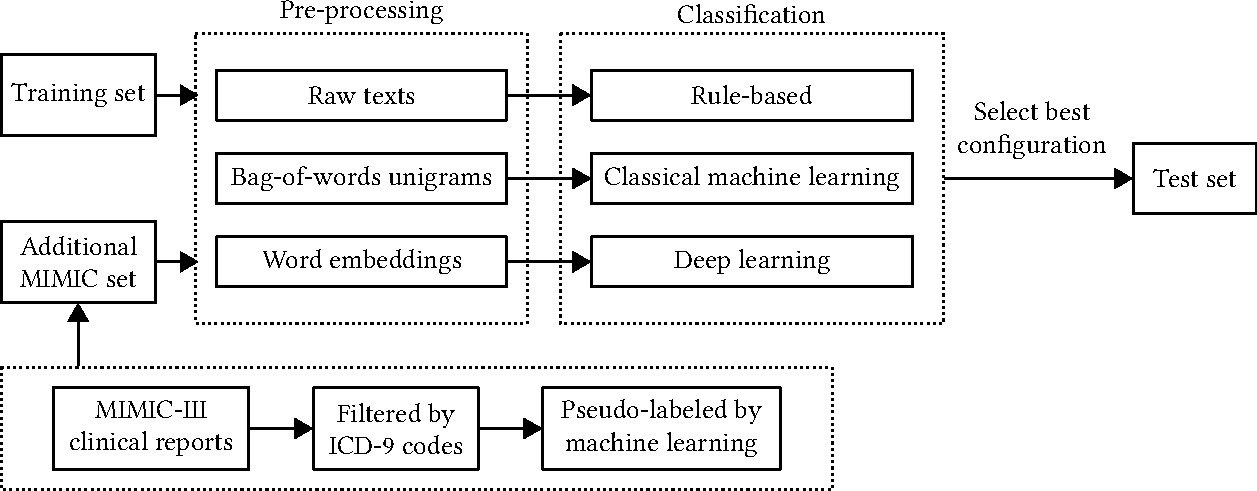
\includegraphics[width=\textwidth]{img/2018-n2c2-system/v4/img.pdf}
\caption{Overall system architecture used in the patient cohort selection task.}
\label{fig:2018-n2c2-system}
\end{center}
\end{figure}



\subsubsection{Overall system}

The system herein described is composed of heuristics and machine learning models.
Our approach consisted in selecting the methods which achieved the best results in the training set and applying them to the test set.
The rule-based methods take as input raw text, while the classical machine learning classifiers use \as{bow} unigrams, and the deep learning models use word embeddings.

In the supervised learning approaches, a few \as{mimic}-III clinical reports were first selected using the \as{icd}-9 codes and then classified considering the probability output by an ensemble classifier pre-trained with the training set in a self-training setting.
The ensemble calculates the average of the probabilities obtained from the five different classical machine learning classifiers.
We tested this setup in the seven tags that were mapped to \as{icd}-9 codes (\Cref{tab:2018-n2c2-icd9}).

\begingroup

% \renewcommand*{\arraystretch}{1.5}
\setlength\tabcolsep{4.1pt}

% \newcommand{\minorscriptsize}{\fontsize{7.0pt}{8.4pt}\selectfont}
\newcommand{\minorfootnotesize}{\fontsize{9.0pt}{10.8pt}\selectfont}

\begin{table}[!tb]

\caption%
[Detailed results with a baseline classifier applied to the 2018 \as{n2c2} Track~1 test set.]%
{Detailed results with a baseline classifier applied to the 2018 \as{n2c2} Track~1 test set. TP: true positive. TN: true negative. FP: false positive. FN: false negative. P:~precision. R: recall. F1: F1-score. MI: micro-averaged. MA: macro-averaged.}%
\label{tab:2018-n2c2-results-baseline}

\centering

% \small
% \footnotesize
\minorfootnotesize
% \scriptsize
% \minorscriptsize
% \tiny

\begin{tabular}{E{6.8mm}T{5mm}T{5mm}T{5mm}T{5mm}T{8mm}T{8mm}T{8mm}T{5mm}T{5mm}T{5mm}T{5mm}T{8mm}T{8mm}T{8mm}T{9mm}}

\toprule

\textbf{Tag}* & \multicolumn{7}{l}{\textbf{Met}} & \multicolumn{7}{l}{\textbf{Not met}} & \textbf{O. F1}\textsuperscript{†}\\

% \cmidrule(r{0.25em}){1-1}\cmidrule(l{0.25em}r{0.25em}){2-8}\cmidrule(l{0.25em}r{0.25em}){9-15}\cmidrule(l{0.25em}){16-16}
\cmidrule(l{0.25em}r{0.25em}){2-8}\cmidrule(l{0.25em}r{0.25em}){9-15}

& TP & TN & FP & FN & P & R & F1 & TP & TN & FP & FN & P & R & F1 &\\

\midrule

\textsf{ABD} &  0 & 56 &  0 & 30 & 0.0000 & 0.0000 & 0.0000 & 56 &  0 & 30 &  0 & 0.6512 & 1.0000 & 0.7887 & 0.3944\\
\textsf{ADV} & 45 &  0 & 41 &  0 & 0.5233 & 1.0000 & 0.6870 &  0 & 45 &  0 & 41 & 0.0000 & 0.0000 & 0.0000 & 0.3435\\
\textsf{ALC} &  0 & 83 &  0 &  3 & 0.0000 & 0.0000 & 0.0000 & 83 &  0 &  3 &  0 & 0.9651 & 1.0000 & 0.9822 & 0.4911\\
\textsf{ASP} & 68 &  0 & 18 &  0 & 0.7907 & 1.0000 & 0.8831 &  0 & 68 &  0 & 18 & 0.0000 & 0.0000 & 0.0000 & 0.4416\\
\textsf{CRE} &  0 & 62 &  0 & 24 & 0.0000 & 0.0000 & 0.0000 & 62 &  0 & 24 &  0 & 0.7209 & 1.0000 & 0.8378 & 0.4189\\
\textsf{DIE} &  0 & 42 &  0 & 44 & 0.0000 & 0.0000 & 0.0000 & 42 &  0 & 44 &  0 & 0.4884 & 1.0000 & 0.6562 & 0.3281\\
\textsf{DRU} &  0 & 83 &  0 &  3 & 0.0000 & 0.0000 & 0.0000 & 83 &  0 &  3 &  0 & 0.9651 & 1.0000 & 0.9822 & 0.4911\\
\textsf{ENG} & 73 &  0 & 13 &  0 & 0.8488 & 1.0000 & 0.9182 &  0 & 73 &  0 & 13 & 0.0000 & 0.0000 & 0.0000 & 0.4591\\
\textsf{HBA} &  0 & 51 &  0 & 35 & 0.0000 & 0.0000 & 0.0000 & 51 &  0 & 35 &  0 & 0.5930 & 1.0000 & 0.7445 & 0.3723\\
\textsf{KET} &  0 & 86 &  0 &  0 & 0.0000 & 0.0000 & 0.0000 & 86 &  0 &  0 &  0 & 1.0000 & 1.0000 & 1.0000 & 0.5000\\
\textsf{MAJ} & 43 &  0 & 43 &  0 & 0.5000 & 1.0000 & 0.6667 &  0 & 43 &  0 & 43 & 0.0000 & 0.0000 & 0.0000 & 0.3333\\
\textsf{MAK} & 83 &  0 &  3 &  0 & 0.9651 & 1.0000 & 0.9822 &  0 & 83 &  0 &  3 & 0.0000 & 0.0000 & 0.0000 & 0.4911\\
\textsf{MI6} &  0 & 78 &  0 &  8 & 0.0000 & 0.0000 & 0.0000 & 78 &  0 &  8 &  0 & 0.9070 & 1.0000 & 0.9512 & 0.4756\\

% ABDOMINAL       %
% ADVANCED-CAD    %
% ALCOHOL-ABUSE   %
% ASP-FOR-MI      %
% CREATININE      %
% DIETSUPP-2MOS   %
% DRUG-ABUSE      %
% ENGLISH         %
% HBA1C           %
% KETO-1YR        %
% MAJOR-DIABETES  %
% MAKES-DECISIONS %
% MI-6MOS         %

\cmidrule(r{0.25em}){1-1}\cmidrule(l{0.25em}r{0.25em}){2-8}\cmidrule(l{0.25em}r{0.25em}){9-15}\cmidrule(l{0.25em}){16-16}

% \textbf{micro-averaged}
% \textbf{macro-averaged}

MI & 312 & 541 & 118 & 147 & 0.7256 & 0.6797 & 0.7019 & 541 & 312 & 147 & 118 & 0.7863 & 0.8209 & 0.8033 & 0.7526\\
MA &     &     &     &     & 0.2791 & 0.3846 & 0.3183 &     &     &     &     & 0.4839 & 0.6154 & 0.5341 & 0.4262\\

\bottomrule

\multicolumn{16}{E{143mm}}{* The names of the tags were abbreviated for conciseness of the table. Please refer to \Cref{tab:2018-n2c2-tags} for consulting the full name forms.}\\
\multicolumn{16}{E{143mm}}{\textsuperscript{†} The overall F1-score is the average between the F1-scores from the `met' and `not met' classes.}

\end{tabular}
\end{table}
\endgroup


Additionally, an optional pre-processing step was developed for the removal of tabular information from text with the aim of limiting document content to natural text.
At the final stage of the pipeline, the pre-processing style, the classifier (heuristics or machine learning), and the training data (with or without additional \as{mimic}-III reports) are chosen so that the best combination is applied to the test set.
\Cref{fig:2018-n2c2-system} shows the final overall system architecture.

Note that for the tag \textsf{KETO-1YR}, the machine learning models were not trained, due to the lack of training samples, being the output pre-defined to always be `not met' in this case.

\begingroup

% \renewcommand*{\arraystretch}{1.7}
% \setlength\tabcolsep{4.6pt}
\setlength\tabcolsep{5.45pt}

\newcommand{\minorfootnotesize}{\fontsize{9.5pt}{11.4pt}\selectfont}
% \newcommand{\minorfootnotesize}{\fontsize{9.0pt}{10.8pt}\selectfont}

\begin{table}[!t]

\caption%
[Overall averaged F1-scores in the 2018 \as{n2c2} Track~1 training and test sets.]%
{\small%
Overall averaged F1-scores in the 2018 \as{n2c2} Track~1 training and test sets. The highest value in each row is highlighted in bold. Ada: \textsf{AdaBoostClassifier}. Bag: \textsf{BaggingClassifier}. DT: \textsf{DecisionTreeClassifier}. GB: \textsf{GradientBoostingClassifier}. XGB: \textsf{XGBClassifier}. FCNN: fully connected neural network. CNN: convolutional neural network. RB: rule-based classifier. MRB: modified rule-based classifier.}
\label{tab:2018-n2c2-results-all}

\centering

% \small
% \footnotesize
\minorfootnotesize
% \scriptsize
% \minorscriptsize
% \tiny

\begin{tabular}{lrrrrrrrrr}

\multicolumn{10}{l}{\small (a) Evaluation on the training set.}\\[4pt]

\toprule

Tag & \multicolumn{5}{l}{Classical machine learning} & \multicolumn{2}{l}{Deep learning} & \multicolumn{2}{l}{Rule-based}\\

\cmidrule(r{0.25em}){1-1}\cmidrule(l{0.25em}r{0.25em}){2-6}\cmidrule(l{0.25em}r{0.25em}){7-8}\cmidrule(l{0.25em}){9-10}

& Ada & Bag & DT & GB & XGB & FCNN & CNN & RB & MRB\\

\textsf{ABDOMINAL}       & \textbf{0.6071} & 0.5024 & 0.5281 & 0.5868          & 0.5654 & 0.5717 & 0.4257 &                 &\\
\textsf{ADVANCED-CAD}    & 0.6780          & 0.6525 & 0.6034 & 0.7208          & 0.7611 & 0.4951 & 0.4977 & \textbf{0.8251} & \textbf{0.8251}\\
\textsf{ALCOHOL-ABUSE}   & 0.4899          & 0.4912 & 0.4807 & 0.4847          & 0.4912 & 0.4912 & 0.4912 &          0.8598 & \textbf{1.0000}\\
\textsf{ASP-FOR-MI}      & 0.5144          & 0.4843 & 0.4946 & 0.5025          & 0.4603 & 0.4466 & 0.4466 &          0.7916 & \textbf{0.8625}\\
\textsf{CREATININE}      & 0.7760          & 0.7959 & 0.7258 & 0.7723          & 0.8042 & 0.4189 & 0.5846 &          0.8895 & \textbf{0.9118}\\
\textsf{DIETSUPP-2MOS}   & 0.6526          & 0.6432 & 0.5937 & 0.6926          & 0.7126 & 0.6539 & 0.5308 & \textbf{0.7975} &\\
\textsf{DRUG-ABUSE}      & 0.7123          & 0.5795 & 0.6802 & 0.7370          & 0.4873 & 0.4873 & 0.4873 & 0.7020          & \textbf{1.0000}\\
\textsf{ENGLISH}         & 0.7780          & 0.7780 & 0.8837 & 0.8837          & 0.5795 & 0.4873 & 0.4873 & 0.9172          & \textbf{1.0000}\\
\textsf{HBA1C}           & 0.5429          & 0.5139 & 0.5588 & 0.5279          & 0.5702 & 0.4568 & 0.4006 & 0.9374          & \textbf{0.9601}\\
\textsf{KETO-1YR}        & 0.5000          & 0.5000 & 0.5000 & 0.5000          & 0.5000 & 0.5000 & 0.5000 & 0.5000          &\\
\textsf{MAJOR-DIABETES}  & 0.7375          & 0.6929 & 0.6554 & \textbf{0.7483} & 0.7429 & 0.5656 & 0.5473 &                 &\\
\textsf{MAKES-DECISIONS} & 0.4873          & 0.4899 & 0.6192 & 0.5706          & 0.4899 & 0.4899 & 0.4899 & 0.8256          & \textbf{1.0000}\\
\textsf{MI-6MOS}         & 0.4753          & 0.5306 & 0.5936 & 0.5097          & 0.5730 & 0.4767 & 0.4767 & 0.8026          & \textbf{0.8778}\\

\cmidrule(r{0.25em}){1-1}\cmidrule(l{0.25em}r{0.25em}){2-6}\cmidrule(l{0.25em}r{0.25em}){7-8}\cmidrule(l{0.25em}){9-10}

Micro-averaged & 0.8198 & 0.8108 & 0.7682 & 0.8222          & \textbf{0.8355} & 0.7813 & 0.7858 & &\\
Macro-averaged & 0.6117 & 0.5888 & 0.6090 & \textbf{0.6336} & 0.5952          & 0.5031 & 0.4897 & &\\

\bottomrule

%%%%%%%%%%%%%%%%%%%%%%%%%%%%%%%%%%%%%%%%%%%%%%%%%%%%%%%%%%%%%%%%%%%%%%%%%%%%%%%%%%%%%%%%%%%%%%%%%%%
%%%%%%%%%%%%%%%%%%%%%%%%%%%%%%%%%%%%%%%%%%%%%%%%%%%%%%%%%%%%%%%%%%%%%%%%%%%%%%%%%%%%%%%%%%%%%%%%%%%
%%%%%%%%%%%%%%%%%%%%%%%%%%%%%%%%%%%%%%%%%%%%%%%%%%%%%%%%%%%%%%%%%%%%%%%%%%%%%%%%%%%%%%%%%%%%%%%%%%%

\\[4pt]

\multicolumn{10}{l}{\small (b) Evaluation on the test set.}\\[4pt]

\toprule

Tag & \multicolumn{5}{l}{Classical machine learning} & \multicolumn{2}{l}{Deep learning} & \multicolumn{2}{l}{Rule-based}\\

\cmidrule(r{0.25em}){1-1}\cmidrule(l{0.25em}r{0.25em}){2-6}\cmidrule(l{0.25em}r{0.25em}){7-8}\cmidrule(l{0.25em}){9-10}

& Ada & Bag & DT & GB & XGB & FCNN & CNN & RB & MRB\\

\textsf{ABDOMINAL}       & 0.7574          & 0.5590          & 0.7079 & \textbf{0.7807} & 0.6334          & 0.4658 & 0.3944 &                 &\\
\textsf{ADVANCED-CAD}    & 0.7977          & 0.7889          & 0.6178 & \textbf{0.8227} & 0.8114          & 0.4113 & 0.6673 & 0.7832          & 0.8089\\
\textsf{ALCOHOL-ABUSE}   & \textbf{0.5896} & 0.4911          & 0.4850 & \textbf{0.5896} & 0.4911          & 0.4911 & 0.4911 & 0.4850          & 0.4850\\
\textsf{ASP-FOR-MI}      & 0.4847          & 0.4401          & 0.5271 & 0.5469          & 0.4908          & 0.4416 & 0.4416 & 0.7095          & \textbf{0.7426}\\
\textsf{CREATININE}      & 0.7329          & 0.7219          & 0.5933 & 0.7219          & 0.7110          & 0.4948 & 0.5411 & \textbf{0.8295} & 0.7862\\
\textsf{DIETSUPP-2MOS}   & 0.6728          & 0.5597          & 0.5930 & 0.6510          & 0.6162          & 0.5390 & 0.5083 & \textbf{0.7943} &\\
\textsf{DRUG-ABUSE}      & 0.4850          & 0.4911          & 0.6815 & 0.6601          & 0.4911          & 0.4911 & 0.4911 & 0.7312          & \textbf{0.9255}\\
\textsf{ENGLISH}         & 0.7559          & \textbf{0.7929} & 0.7915 & 0.7929          & 0.5983          & 0.4591 & 0.4591 & 0.6554          & 0.6554\\
\textsf{HBA1C}           & 0.6098          & 0.6048          & 0.6210 & 0.5773          & 0.5773          & 0.3676 & 0.3723 & \textbf{0.9382} & 0.8439\\
\textsf{KETO-1YR}        & 0.5000          & 0.5000          & 0.5000 & 0.5000          & 0.5000          & 0.5000 & 0.5000 & 0.4971          &\\
\textsf{MAJOR-DIABETES}  & 0.7902          & 0.8023          & 0.6975 & \textbf{0.8721} & 0.8023          & 0.6044 & 0.5966 &                 &\\
\textsf{MAKES-DECISIONS} & 0.4911          & 0.4881          & 0.6277 & 0.4850          & \textbf{0.7440} & 0.4911 & 0.4911 & 0.6067          & 0.4911\\
\textsf{MI-6MOS}         & 0.4724          & 0.4756          & 0.4625 & 0.4724          & 0.4756          & 0.4756 & 0.4756 & 0.7281          & \textbf{0.8102}\\

\cmidrule(r{0.25em}){1-1}\cmidrule(l{0.25em}r{0.25em}){2-6}\cmidrule(l{0.25em}r{0.25em}){7-8}\cmidrule(l{0.25em}){9-10}

Micro-averaged & 0.8331 & 0.8134 & 0.7775 & \textbf{0.8356} & 0.8258 & 0.7566 & 0.7676 & &\\
Macro-averaged & 0.6261 & 0.5935 & 0.6081 & \textbf{0.6517} & 0.6110 & 0.4794 & 0.4946 & &\\

\bottomrule

\end{tabular}
\end{table}
\endgroup



\subsection{Results and discussion}

In this section, we present several results obtained by applying different methods in the training and test sets.
Performance in the training set was evaluated using 3-fold cross-validation in the case of supervised learning algorithms, whereas the rule-based classifiers were applied directly to the complete training set because they did not need to learn from labeled training samples.

We used two evaluation metrics proposed by the \as{n2c2} organizers which take into account the dataset imbalance: overall micro- and macro-averaged F1-scores.
This overall score is the average of the two F1-scores of the `met' and `not met' classes.
The evaluation metrics were calculated for each tag, thus enabling the analysis of each criterion separately.

\begingroup

% \renewcommand*{\arraystretch}{1.5}
\setlength\tabcolsep{4.2pt}

% \newcommand{\minorfootnotesize}{\fontsize{9.5pt}{11.4pt}\selectfont}
\newcommand{\minorfootnotesize}{\fontsize{9.4pt}{11.28pt}\selectfont}
% \newcommand{\minorfootnotesize}{\fontsize{9.0pt}{10.8pt}\selectfont}

\begin{table}[!t]

\caption%
[Overall averaged F1-scores in the 2018 \as{n2c2} Track~1 dataset with classifiers trained with 100~additional `met' training \as{mimic}-III reports.]%
{Overall averaged F1-scores in the 2018 \as{n2c2} Track~1 dataset with classifiers trained with 100~additional `met' training \as{mimic}-III reports. The highest value for each tag and subset is highlighted in bold. Ada: \textsf{AdaBoostClassifier}. Bag: \textsf{BaggingClassifier}. DT: \textsf{DecisionTreeClassifier}. GB: \textsf{GradientBoostingClassifier}. XGB: \textsf{XGBClassifier}.}
\label{tab:2018-n2c2-results-mimic100p}

\centering

% \small
% \footnotesize
\minorfootnotesize
% \scriptsize
% \minorscriptsize
% \tiny

\begin{tabular}{lrrrrrrrrrr}

\toprule

Tag & \multicolumn{5}{l}{Evaluation on the training set} & \multicolumn{5}{l}{Evaluation on the test set}\\

\cmidrule(r{0.25em}){1-1}\cmidrule(l{0.25em}r{0.25em}){2-6}\cmidrule(l{0.25em}){7-11}

& Ada & Bag & DT & GB & XGB & Ada & Bag & DT & GB & XGB\\

% \midrule

\textsf{ABDOMINAL}      & \textbf{0.6669} & 0.5890          & 0.6075 & 0.6655          & 0.6581 & 0.7511          & \textbf{0.7617} & 0.6595          & 0.7352          & 0.7507\\
\textsf{ALCOHOL-ABUSE}  & 0.6729          & \textbf{0.7949} & 0.7040 & 0.7040          & 0.7159 & \textbf{0.5753} & 0.4911          & 0.4819          & 0.4911          & 0.4911\\
\textsf{ASP-FOR-MI}     & \textbf{0.5848} & 0.5365          & 0.4976 & 0.4951          & 0.4873 & 0.4673          & 0.5232          & \textbf{0.5784} & 0.4788          & 0.4379\\
\textsf{DIETSUPP-2MOS}  & 0.6977          & 0.6781          & 0.6219 & \textbf{0.7335} & 0.7106 & 0.6012          & 0.6007          & 0.5697          & 0.6510          & \textbf{0.6977}\\
\textsf{DRUG-ABUSE}     & \textbf{0.7228} & 0.7093          & 0.6456 & 0.6962          & 0.7093 & \textbf{0.7440} & 0.6910          & 0.6601          & 0.6815          & \textbf{0.7440}\\
\textsf{MAJOR-DIABETES} & 0.7335          & 0.7214          & 0.6231 & \textbf{0.7537} & 0.7489 & 0.7790          & 0.6512          & 0.7089          & \textbf{0.8372} & 0.8140\\
\textsf{MI-6MOS}        & 0.6930          & \textbf{0.7023} & 0.7020 & 0.6842          & 0.6842 & \textbf{0.4724} & \textbf{0.4724} & 0.4625          & \textbf{0.4724} & \textbf{0.4724}\\

\bottomrule

\end{tabular}
\end{table}
\endgroup


For a clear understanding and detailed exposition of all the calculated metrics, \Cref{tab:2018-n2c2-results-baseline} presents the results from a baseline classifier which simply attributed the most frequent label in the training set to all test samples.
This baseline classifier attained a micro-F1 of~0.7526 and a macro-F1 of~0.4262 on the test set.
To simplify the presentation of the results, we only present the overall F1-scores in the next experiments.
However, detailed results containing true positive, true negative, false positive, and false negative counts as presented in \Cref{tab:2018-n2c2-results-baseline}, were examined during the refinement of our approach.

\Cref{tab:2018-n2c2-results-all} shows the results of machine learning and rule-based methods evaluated on the (a) training and (b) test sets.
Looking only at the evaluation in the training set, one can see that for each tag where rules were implemented, the rule-based method was the best performing classifier.
On the other hand, deep learning models produced the worst results.

\begingroup

% \renewcommand*{\arraystretch}{1.6}
\setlength\tabcolsep{4.05pt}

% \newcommand{\minorfootnotesize}{\fontsize{9.5pt}{11.4pt}\selectfont}
% \newcommand{\minorfootnotesize}{\fontsize{9.4pt}{11.28pt}\selectfont}
% \newcommand{\minorfootnotesize}{\fontsize{9.3pt}{11.16pt}\selectfont}
\newcommand{\minorfootnotesize}{\fontsize{9.2pt}{11.04pt}\selectfont}
% \newcommand{\minorfootnotesize}{\fontsize{9.0pt}{10.8pt}\selectfont}

\begin{table}[!t]

\caption%
[Overall averaged F1-scores in the 2018 \as{n2c2} Track~1 dataset with tabulated information removed from the raw texts.]%
{Overall averaged F1-scores in the 2018 \as{n2c2} Track~1 dataset with tabulated information removed from the raw texts. The highest value for each row and subset is highlighted in bold. Ada: \textsf{AdaBoostClassifier}. Bag: \textsf{BaggingClassifier}. DT: \textsf{DecisionTreeClassifier}. GB: \textsf{GradientBoostingClassifier}. XGB: \textsf{XGBClassifier}.}
\label{tab:2018-n2c2-results-notabular}

\centering

% \small
% \footnotesize
\minorfootnotesize
% \scriptsize
% \minorscriptsize
% \tiny

\begin{tabular}{lrrrrrrrrrr}

\toprule

Tag & \multicolumn{5}{l}{Evaluation on the training set} & \multicolumn{5}{l}{Evaluation on the test set}\\

\cmidrule(r{0.25em}){1-1}\cmidrule(l{0.25em}r{0.25em}){2-6}\cmidrule(l{0.25em}){7-11}

& Ada & Bag & DT & GB & XGB & Ada & Bag & DT & GB & XGB\\

\textsf{ABDOMINAL}       & \textbf{0.6325} & 0.5466          & 0.5676          & 0.5957          & 0.5733          & 0.7399          & 0.5419          & 0.6765          & \textbf{0.8294} & 0.6052\\
\textsf{ADVANCED-CAD}    & 0.6668          & 0.6952          & 0.5761          & \textbf{0.7405} & \textbf{0.7405} & 0.8089          & 0.7531          & 0.6549          & \textbf{0.8350} & \textbf{0.8350}\\
\textsf{ALCOHOL-ABUSE}   & 0.4899          & \textbf{0.4912} & 0.4794          & 0.4847          & \textbf{0.4912} & \textbf{0.5753} & 0.4911          & \textbf{0.5753} & \textbf{0.5753} & 0.4911\\
\textsf{ASP-FOR-MI}      & 0.5064          & 0.5076          & \textbf{0.5190} & 0.5084          & 0.4603          & 0.4908          & 0.4454          & \textbf{0.5947} & 0.5086          & 0.4342\\
\textsf{CREATININE}      & 0.7726          & 0.7726          & 0.6966          & 0.7864          & \textbf{0.7978} & 0.6718          & 0.6946          & 0.6142          & 0.7141          & \textbf{0.7329}\\
\textsf{DIETSUPP-2MOS}   & 0.6261          & 0.6574          & 0.6081          & 0.6631          & \textbf{0.6830} & \textbf{0.7089} & 0.6073          & 0.5216          & 0.6158          & 0.6728\\
\textsf{DRUG-ABUSE}      & \textbf{0.7123} & 0.4873          & 0.5825          & 0.7093          & 0.4873          & 0.4819          & 0.4911          & \textbf{0.6601} & \textbf{0.6601} & 0.4911\\
\textsf{ENGLISH}         & 0.7780          & \textbf{0.9079} & 0.8422          & 0.8837          & 0.5795          & 0.7559          & \textbf{0.7929} & 0.7737          & \textbf{0.7929} & 0.5983\\
\textsf{HBA1C}           & \textbf{0.6087} & 0.5568          & 0.5462          & 0.5216          & 0.5816          & \textbf{0.5951} & 0.4574          & 0.5232          & 0.5681          & 0.5577\\
\textsf{KETO-1YR}        & 0.5000          & 0.5000          & 0.5000          & 0.5000          & 0.5000          & 0.5000          & 0.5000          & 0.5000          & 0.5000          & 0.5000\\
\textsf{MAJOR-DIABETES}  & 0.7637          & 0.6859          & 0.6354          & \textbf{0.7725} & 0.7094          & 0.7906          & 0.7673          & 0.6510          & \textbf{0.8604} & 0.8136\\
\textsf{MAKES-DECISIONS} & 0.4873          & 0.4899          & \textbf{0.5629} & 0.4886          & 0.4899          & 0.4881          & 0.4911          & 0.6546          & 0.4850          & \textbf{0.7440}\\
\textsf{MI-6MOS}         & 0.4753          & 0.5306          & 0.5601          & 0.5097          & \textbf{0.5730} & 0.4724          & \textbf{0.4756} & 0.4658          & 0.4724          & \textbf{0.4756}\\

\cmidrule(r{0.25em}){1-1}\cmidrule(l{0.25em}r{0.25em}){2-6}\cmidrule(l{0.25em}){7-11}

Micro-averaged & 0.8270 & 0.8185 & 0.7657 & 0.8263          & \textbf{0.8306} & 0.8298 & 0.8031 & 0.7675 & \textbf{0.8336} & 0.8304\\
Macro-averaged & 0.6169 & 0.6022 & 0.5905 & \textbf{0.6280} & 0.5897          & 0.6215 & 0.5776 & 0.6051 & \textbf{0.6475} & 0.6117\\

\bottomrule

\end{tabular}
\end{table}
\endgroup


The \textsf{AdaBoostClassifier} and the \textsf{GradientBoostingClassifier} achieved the two highest macro-average F1-scores both in training and test sets.
For the tags where the modified rule-based classifier was implemented, this classifier achieved the best results in the training set, but the same was not verified for the test set which shows that certain rules were overfit to the training set.
For the tags \textsf{ABDOMINAL}, \textsf{ADVANCED-CAD}, and \textsf{MAJOR-DIABETES}, the results obtained with classical machine learning significantly improved in the test set proving that training with more data helped to increase their generalization ability.

\begingroup

\newcommand{\methodA}{\textsf{AdaBoostClassifier} with 100 additional training \as{mimic} reports}
\newcommand{\methodB}{Rule-based classifier}
\newcommand{\methodC}{Modified rule-based classifier}
\newcommand{\methodD}{Modified rule-based classifier}
\newcommand{\methodE}{Modified rule-based classifier}
\newcommand{\methodF}{Rule-based classifier}
\newcommand{\methodG}{Modified rule-based classifier}
\newcommand{\methodH}{Modified rule-based classifier}
\newcommand{\methodI}{Modified rule-based classifier}
\newcommand{\methodJ}{Rule-based classifier}
\newcommand{\methodK}{\textsf{GradientBoostingClassifier} with tabulated information discarded}
\newcommand{\methodL}{Modified rule-based classifier}
\newcommand{\methodM}{Modified rule-based classifier}

% \renewcommand*{\arraystretch}{1.5}
\setlength\tabcolsep{4.0pt}

\newcommand{\minorfootnotesize}{\fontsize{9.5pt}{11.4pt}\selectfont}
% \newcommand{\minorfootnotesize}{\fontsize{9.4pt}{11.28pt}\selectfont}
% \newcommand{\minorfootnotesize}{\fontsize{9.3pt}{11.16pt}\selectfont}
% \newcommand{\minorfootnotesize}{\fontsize{9.2pt}{11.04pt}\selectfont}
% \newcommand{\minorfootnotesize}{\fontsize{9.0pt}{10.8pt}\selectfont}

\begin{table}[!t]

\caption%
[Overall averaged F1-scores in the 2018 \as{n2c2} Track~1 dataset with the best combination of methods selected by inspecting the evaluation in the training set.]%
{Overall averaged F1-scores in the 2018 \as{n2c2} Track~1 dataset with the best combination of methods selected by inspecting the evaluation in the training set. The methods that provided the best results in the training set were applied. The highest value for each tag is highlighted in bold.}
\label{tab:2018-n2c2-results-best-configuration}

\centering

% \small
% \footnotesize
\minorfootnotesize
% \scriptsize
% \minorscriptsize
% \tiny

\begin{tabular}{llrr}

\toprule

Selected method & Tag & \multicolumn{1}{l}{Training} & \multicolumn{1}{l}{Test}\\

\cmidrule(r{0.25em}){1-1}\cmidrule(l{0.25em}r{0.25em}){2-2}\cmidrule(l{0.25em}r{0.25em}){3-3}\cmidrule(l{0.25em}){4-4}

% \midrule

\methodA & \textsf{ABDOMINAL}       & 0.6669          & \textbf{0.7511}\\
\methodB & \textsf{ADVANCED-CAD}    & \textbf{0.8251} & 0.8089\\
\methodC & \textsf{ALCOHOL-ABUSE}   & \textbf{1.0000} & 0.4850\\
\methodD & \textsf{ASP-FOR-MI}      & \textbf{0.8625} & 0.7426\\
\methodE & \textsf{CREATININE}      & \textbf{0.9118} & 0.7862\\
\methodF & \textsf{DIETSUPP-2MOS}   & \textbf{0.7975} & 0.7943\\
\methodG & \textsf{DRUG-ABUSE}      & \textbf{1.0000} & 0.9255\\
\methodH & \textsf{ENGLISH}         & \textbf{1.0000} & 0.6554\\
\methodI & \textsf{HBA1C}           & \textbf{0.9601} & 0.8439\\
\methodJ & \textsf{KETO-1YR}        & \textbf{0.5000} & 0.4971\\
\methodK & \textsf{MAJOR-DIABETES}  & 0.7725          & \textbf{0.8604}\\
\methodL & \textsf{MAKES-DECISIONS} & \textbf{1.0000} & 0.4911\\
\methodM & \textsf{MI-6MOS}         & \textbf{0.8778} & 0.8102\\

\cmidrule(l{0.25em}r{0.25em}){2-2}\cmidrule(l{0.25em}r{0.25em}){3-3}\cmidrule(l{0.25em}){4-4}

& Micro-averaged & \textbf{0.9143} & 0.8844\\
& Macro-averaged & \textbf{0.8596} & 0.7271\\

\bottomrule

\end{tabular}
\end{table}
\endgroup


\Cref{tab:2018-n2c2-results-mimic100p} shows the results when 100~additional `met' \as{mimic}-III reports are used for training.
Because these additional reports were classified with pre-trained models on the full training dataset, these results are indirectly biased.
This explains the fact that the results in the training set have more noticeable improvements, whereas the improvements in the test set are less significant, in comparison to the original results from \Cref{tab:2018-n2c2-results-all}.

\Cref{tab:2018-n2c2-results-notabular} presents the results obtained when applying classical machine learning with tabulated information removed from the raw texts. Significant differences were not found when compared to the results presented in \Cref{tab:2018-n2c2-results-all}.

Finally, \Cref{tab:2018-n2c2-results-best-configuration} shows the final results when the best combination was selected by inspecting the results in the training set.
The best combination in the training set achieved a micro-F1 of 0.9143 and a macro-F1 of 0.8596 whereas in the test set it attained a micro-F1 of 0.8844 and a macro-F1 of 0.7271.
These results show that there is a clear overfitting to the training set because the macro-F1 on the test set is around 13 percentage points lower.
We highlight that, in this optimal configuration, rule-based methods were mostly selected.

Our system contains rule-based methods and machine learning algorithms that are accordingly selected to better classify each criterion.
We developed handcrafted rules for almost all the criteria.
However, the process of creating adequate rules is hard and cumbersome since it requires an analysis of the data, not excluding the medical expertise that is oftentimes required.
Moreover, while rule-based methods achieved good results, these require the development of a distinct algorithm for each criterion while machine learning classifiers do not face this problem, being easier to re-use.

In this task, classical machine learning classifiers worked much better when compared to deep learning classifiers.
In most cases, deep learning models predicted the same label for every sample, behaving similarly to a baseline classifier and demonstrating that the dataset had a reduced size.
Our results also show that machine learning classifiers provided better results for criteria with balanced labels, evidencing that other criteria lack in training data.


\section{Measuring clinical semantic textual similarity}
\label{c4:s:clinical-sts}

For years, technology advancements have been applied in health care with the goal of preventing, diagnosing and treating diseases, as well as improving the quality of life of the general population.
These technological breakthroughs have brought new tools and information sources to physicians, aiding them in clinical workflows like patient follow-up and clinical decision making, whilst also playing an important role in the transition into the personalized medicine paradigm.

Electronic health records are an example of such widely adopted technologies in medicine, providing an electronic infrastructure that can aggregate a multitude of medical information and support the medical act.
\asp{ehr} provide a longitudinal view of patient trajectory comprehending the past and present of a patient's health condition, and can also comprehend a future component of the patient trajectory if future treatments and appointments are considered.
Despite these containing rich contextual information in structured data that could for instance be explored for prediction modelling purposes \parencite{wu2010a,ferrao2013a,ferrao2016a}, large amounts of valuable patient information are stored in unstructured notes, commonly referred to as free text, which are often underexplored due to difficulties in processing this type of text \parencite{neustein2014a}.

Due to the large extent of information contained in an \as{ehr}, physicians are provided with the key aspect of \textit{context} when reasoning on their medical decisions, making \as{ehr} a key component of the patient-centered notion of health care.
However, even though its wide adoption has enabled an improvement on healthcare quality, certain challenges also arose with it.
An example of such issue is the facilitated process of replicating information in medical text reports through copy-paste actions or by using pseudo-templates.
This has impacted on \as{ehr} data quality since it can lead to less concise documentation, and an increased chance of introducing erroneous information, that can consequently compromise the quality of the medical act \parencite{cohen2013a,singh2013a}.

Due to the importance of reducing the dimension and redundancy in \as{ehr} data, solutions for annotating relevant data and summarizing clinical text \parencite{pivovarov2015a} have been the focus of much research, mostly targeting clinical natural language processing.
A possible recently explored approach to reduce clinical text redundancy is by assessing the semantic textual similarity between different text excerpts from an \as{ehr}.
Investigation on semantic textual similarity has attracted particular attention in past years.
SemEval, an ongoing series of evaluations of computational semantic analysis systems, started a pilot \as{sts} challenge track in 2012 which attracted the attention of the research community~\parencite{agirre2012a} and, due to its success, progressively organized a series of \as{sts} challenge tracks from 2012 through 2017~\parencite{agirre2013a,agirre2014b,agirre2015a,agirre2016a,cer2017a}.
However, these shared tasks had the major drawback of being centered in general-domain text, whereas clinical text is inherently different in its characteristics.
Therefore, an additional effort for the clinical domain was required.

The increasing interest in exploring and pushing forward existing research with clinical data, to further improve healthcare quality, led to the creation of dedicated resources and challenges. To that extent, in recent years, text corpora specifically focused on clinical text were created along with shared tasks on clinical \as{sts} that leverage from those corpora.

In this section we present an approach to measure the semantic textual similarity between clinical sentences.
We explore neural networks and different types of text pre-processing pipelines, and evaluate the impact of using word embeddings or sentence embeddings.
We present our results on the 2019 \as{n2c2}/\as{ohnlp} Track~1 shared task\footnote{\url{https://portal.dbmi.hms.harvard.edu/projects/n2c2-2019-t1/}} dataset, perform an error analysis, and discuss obtained results along with possible future improvements.


\subsubsection{Biomedical and clinical \as{sts} resources}

Recent years have shown efforts to bring \as{sts} to the clinical domain.
Motivated by the rapidly increasing availability of textual data in the biomedical domain, by the need to facilitate the retrieval and analysis of this data, and also by the lack of suitable datasets for the development of appropriate systems, \textcite{sogancioglu2017a} created BIOSSES---a benchmark dataset containing 100~sentence pairs from biomedical literature where each sentence pair was scored in a scale from~0 to~4 regarding its semantic similarity.
Despite being an interesting initial effort, as the type of text found in biomedical literature significantly differs from that of medical narratives, an additional effort was still required.

With the goal of exploring \as{sts} to reduce clinical text redundancy, \textcite{wang2018d} assembled the MedSTS dataset containing 174\,629~pairs of clinical sentences extracted from a clinical corpus at Mayo Clinic.
From this pool of clinical sentence pairs, 1068~pairs were annotated by two medical experts regarding their semantic similarity, who classified each pair with a value within 0 (dissimilar) and 5 (equivalent), resulting in the creation of the MedSTS\_ann dataset.
The authors used MedSTS\_ann to compare the performance of existing \as{sts} approaches on general and clinical domain \as{sts} datasets, and as expected they observed that performances obtained on MedSTS\_ann were in general lower, demonstrating the higher complexity of clinical text.


\subsubsection{Clinical \as{sts} shared tasks}

Driven by the interest of motivating the research community to solve real world clinical problems, \textcite{wang2018e} organized a shared task on clinical \as{sts} where they released MedSTS\_ann, hence making it the first available resource for the study of clinical \as{sts}.
The pioneering shared task was titled BioCreative/\as{ohnlp} Challenge 2018 Task~2: Clinical Semantic Textual Similarity\footnote{\url{https://sites.google.com/view/ohnlp2018/home}} and attracted the participation of four teams who developed automatic systems to measure the semantic relation of sentence pairs from MedSTS\_ann.

Submitted solutions explored various techniques ranging from conventional machine learning to deep learning models.
The winning system \parencite{chen2018d} used a regression model that evaluates the scores obtained by eight trained models based on traditional machine learning and neural networks using sentence encoders.
This system attained the highest Pearson correlation of 0.8328.
The second placing team \parencite{xiong2018a} obtained its best correlation result (0.8143) with an ensemble that combined the predictions from an attention-based \as{cnn} and a bidirectional \as{lstm} models.
The third team \parencite{liu2018c} used sentence embeddings by performing a weighted average of word vectors and obtained a Pearson correlation of 0.7789.
The final team attained a best Pearson correlation of 0.7090 and did not disclose a detailed approach.

On a more recent note, building upon the experience from the BioCreative/\as{ohnlp} shared task on clinical \as{sts}, a collaboration between \as{n2c2} and \as{ohnlp} resulted in the 2019 \as{n2c2}/\as{ohnlp} Track~1 on clinical semantic textual similarity \parencite{wang2020d} with the objective of expanding previous work by providing novel annotated data, thus allowing further development and evaluation of systems on previously unseen data.


\subsubsection{Sentence representation: BioWordVec \versus\ BioSentVec}

Posterior to the BioCreative/\as{ohnlp} shared task, members from the winning team proceeded their work by exploring the field of sentence representation, focusing on word and sentence embeddings.
Due to the limitations of traditional word embeddings, which are computed at the word-level and trained for general-domain text, \textcite{zhang2019c} decided to develop a set of biomedical word embeddings that combined subword information from biomedical text with the biomedical vocabulary \as{mesh}.
The resulting biomedical word embeddings, named BioWordVec, performed better than word2vec embeddings in medical word pair similarity benchmarks, and were made publicly available to the community.
The authors further improved these embeddings by training them on a new corpus containing over 30~million documents from \as{pubmed} articles and clinical notes from the \as{mimic}-III clinical database.

Word embeddings capture representations at word-level, thus to represent a sentence it is necessary to decompose it in words and combine the representations from each word.
However, it is also possible to represent sentence text in a more straightforward approach, using instead sentence embeddings.
Similarly to the word embeddings scenario, despite the existence of pre-trained sentence encoders for the general-domain, biomedical and clinical text remained an unexplored field, thus \textcite{chen2019g} trained a sentence embeddings model on the same dataset, combining \as{pubmed} and \as{mimic}-III text data, used for BioWordVec.
The result was BioSentVec\footnote{\url{https://github.com/ncbi-nlp/BioSentVec}}, a publicly available sentence embeddings model suitable for biomedical and clinical text applications.

To assess the adequacy and effectiveness of these sentence embeddings, \textcite{chen2019g} tested BioSentVec with BIOSSES and MedSTS\_ann.
Whilst using a much simpler 5-layer deep learning model that only received two sentence vectors generated by BioSentVec as input, the authors managed to obtain a Pearson correlation of~0.836 in MedSTS\_ann, slightly improving the previous state-of-the-art.
This demonstrated that BioSentVec embeddings can effectively capture sentence semantics in clinical text.
The authors performed a further comparative evaluation in MedSTS\_ann using various sentence similarity models, including the latest bidirectional transformers in the clinical domain, such as BioBERT \parencite{lee2020a}, and observed that (1) their simpler approach still obtained the best performance, and (2) embeddings trained on large corpora are the best solution to capture sentence semantics in small datasets \parencite{chen2019a}.


\subsection{Materials and methods}

In this work we evaluate a machine learning system in a supervised setting for predicting the semantic relatedness between clinical sentences.
For this task, a real value in the interval [0,~5] is attributed to each pair of sentences: if two sentences are completely unrelated they have a similarity score of~0 (minimum); otherwise if they share the same semantic meaning their similarity value is~5 (maximum).
Alike previous challenges on \as{sts} \parencite{wang2018e,cer2017a} the evaluation metric is the Pearson correlation coefficient, where two lists of similarity values---system predictions and ground-truth---are compared.

In the following sections we describe the dataset used in this work, the different approaches used to pre-processing clinical text, the process of feature representation, and finally the deep learning models employed in our simulations.


\subsubsection{Dataset}

The dataset contained a total of 2054 sentence pairs, and it was beforehand split by the \as{n2c2}~organizers into training and test subsets.
The training data allowed for model development, whereas the test data was used solely for official evaluation in the challenge.
Only afterwards, the ground-truth scores of the test set were made available to the participating teams.
\Cref{tab:2019-n2c2-dataset} presents some statistics about the dataset.
Surprisingly, the distribution of the similarity scores between the two subsets (training and test) are somewhat discrepant since the test data contains a higher number of pairs with scores in the interval~[0,~1].

A list of example clinical sentence pairs is provided in \Cref{tab:2019-n2c2-examples}, containing the sentence pairs, their respective similarity score, and an explanation of the criteria used to assign the score.

\begingroup
\newcommand{\z}{\hphantom{]}}

% \renewcommand{\arraystretch}{1.4}

\begin{table}[!tb]

\caption%
[Statistics of the 2019 \as{n2c2}/\as{ohnlp} Track~1 dataset detailing the number of pairs for different levels of similarity.]%
{Statistics of the 2019 \as{n2c2}/\as{ohnlp} Track~1 dataset detailing the number of pairs for different levels of similarity. N: number of sentence pairs.}%
\label{tab:2019-n2c2-dataset}

\centering

% \small
% \footnotesize
% \scriptsize
% \tiny

\begin{tabular}{lE{0mm}rE{0mm}rrrrr}

\toprule

Set & & \multicolumn{1}{l}{N} & & \multicolumn{5}{l}{Similarity scores}\\

% \midrule
% \cmidrule(r){1-1}\cmidrule(lr){2-2}\cmidrule(l){3-7}
\cmidrule{1-1}\cmidrule{3-3}\cmidrule{5-9}

& & & & [0, 1] & ]1, 2] & ]2, 3] & ]3, 4] & ]4, 5]\\

% \midrule

Training & & 1642 & & 312\z & 154\z & 394\z & 509\z & 273\z\\
Test     & &  412 & & 238\z &  46\z &  32\z &  62\z &  34\z\\

% \midrule
% \cmidrule(r){1-1}\cmidrule(lr){2-2}\cmidrule(l){3-7}
\cmidrule{1-1}\cmidrule{3-3}\cmidrule{5-9}

Total    & & 2054 & & 550\z & 200\z & 426\z & 571\z & 307\z\\

\bottomrule

\end{tabular}
\end{table}
\endgroup

\begingroup

% \renewcommand{\arraystretch}{1.4}
% \renewcommand{\arraystretch}{1.0}

\begin{table}[!tb]

\caption%
[Examples of clinical sentence pairs and respective similarity scores.]%
{Examples of clinical sentence pairs and respective similarity scores with explanations from \textcite{wang2018d}.}%
\label{tab:2019-n2c2-examples}

\centering

% \small
\footnotesize
% \scriptsize
% \tiny

\begin{tabular}{R{8.4mm}E{6.0mm}@{\hskip0pt}E{123mm}}

\toprule

Score & \multicolumn{2}{l}{Examples}\\

\midrule

5 & \multicolumn{2}{E{129mm}}{\textit{The two sentences are completely equivalent, as they mean the same thing.}}\\
& S1: & Albuterol [PROVENTIL/VENTOLIN] 90 mcg/Act HFA Aerosol 2 puffs by inhalation every 4 h as needed\\
& S2: & Albuterol [PROVENTIL/VENTOLIN] 90 mcg/Act HFA Aerosol 1-2 puffs by inhalation every 4 h as needed \#1 each\\

&&\\[-10pt]

4 & \multicolumn{2}{E{129mm}}{\textit{The two sentences are mostly equivalent, but some unimportant details differ.}}\\
& S1: & Discussed goals, risks, alternatives, advanced directives, and the necessity of other members of the surgical team participating in the procedure with the patient\\
& S2: & Discussed risks, goals, alternatives, advance directives, and the necessity of other members of the healthcare team participating in the procedure with the patient and his mother\\

&&\\[-10pt]

3 & \multicolumn{2}{E{129mm}}{\textit{The two sentences are roughly equivalent, but some important information differs or is missing.}}\\
& S1: & Cardiovascular assessment findings include heart rate normal, Heart rhythm, atrial fibrillation with controlled ventricular response\\
& S2: & Cardiovascular assessment findings include heart rate, bradycardic, Heart rhythm, first degree AV Block\\

&&\\[-10pt]

2 & \multicolumn{2}{E{129mm}}{\textit{The two sentences are not equivalent, but share some details.}}\\
& S1: & Discussed risks, goals, alternatives, advance directives, and the necessity of other members of the healthcare team participating in the procedure with (patient) (legal representative and others present during the discussion)\\
& S2: & We discussed the low likelihood that a blood transfusion would be required during the postoperative period and the necessity of other members of the surgical team participating in the procedure\\

&&\\[-10pt]

1 & \multicolumn{2}{E{129mm}}{\textit{The two sentences are not equivalent, but are on the same topic.}}\\
& S1: & No: typical `cold' symptoms; fever present (greater than or equal to 100.4 ºF or 38 ºC) or suspected fever; rash; white patches on lips, tongue or mouth
(other than throat); blisters in the mouth; swollen or `bull' neck; hoarseness or lost voice or ear pain\\
& S2: & New wheezing or chest tightness, runny or blocked nose, or discharge down the back of the throat, hoarseness or lost voice\\

&&\\[-10pt]

0 & \multicolumn{2}{E{129mm}}{\textit{The two sentences are completely dissimilar.}}\\
& S1: & The risks and benefits of the procedure were discussed, and the patient consented to this procedure\\
& S2: & The content of this note has been reproduced, signed by an authorized physician in the space above, and mailed to the patient's parents, the patient's home care company\\

\bottomrule

\end{tabular}
\end{table}
\endgroup



\subsubsection{Clinical text pre-processing}

Before converting sentences into embedding representations, it was necessary to apply a pre-processing step to the clinical sentence pairs.
In this work, three different pipelines were tested.


\paragraph{Base pre-processing}

The baseline pre-processing pipeline was simple, consisting only of two steps: (1) lowercase conversion of the text, and (2) tokenization using the \as{nltk} tokenizer\footnote{\url{https://www.nltk.org/}}.


\paragraph{Advanced pre-processing with full stop word removal}

This pipeline was inspired on the pre-processing used by \textcite{chen2018d} in the BioCreative/\as{ohnlp} 2018 Task on Clinical Semantic Textual Similarity, and had the objective of retaining as much semantic information as possible in pre-processed sentences.

The pipeline started with the separation of number ranges (0.3-1.8 $\rightarrow$ 0.3 to 1.8) which are frequent in lab analysis data.
The second step was to extend numbers into their textual counterpart (78 $\rightarrow$ seventy-eight; 0.9 $\rightarrow$ zero point nine).
Next, words connected with slashes, dashes and dots where separated with spaces (yes/no $\rightarrow$ yes / no; point-of-care $\rightarrow$ point - of - care).
Then starting white spaces are removed, and consecutive spaces are converted to single spaces.

The resulting text is converted to lowercase and tokenized with the \as{nltk} tokenizer.
Finally, a stop word removal is performed using a complete stop word list for biomedical literature\footnote{\url{https://www.ncbi.nlm.nih.gov/IRET/DATASET}}, punctuation is removed from the tokens, and tokens composed of a single character are discarded.


\paragraph{Advanced pre-processing with partial stop word removal}

This approach is similar to the previous processing pipeline, differing only in the stop word removal part.
Since the list of stop words for biomedical text contains terms that can be important for retaining the semantics in clinical text, a smaller stop word list from \textcite{luo2019a} was used instead, being composed of the following terms: 's, a, an, any, her, his, patient, that, the, these, this, those, your.


\subsubsection{Feature representation}

A crucial step in machine learning is feature representation, which aims to transform any kind of data (text, image, and others) into a numeric representation.
For this clinical \as{sts} task we evaluated, separately, the use of word embeddings and sentence embeddings.
We employed the publicly available BioWordVec and BioSentVec models created by \textcite{chen2019g}.
To encode the sentences using word embeddings we normalized the sum of the embedding vectors of their constituent words.


\subsubsection{Deep learning model}

The Keras library \parencite{chollet2015a} was used to implement and test different neural network models.
Our proposed model was derived from other state-of-the-art works \parencite{chen2019g,chen2018d} that use word and sentence embeddings.
We tested various types and configurations of deep learning models, yet simpler models yielded better results, similarly to what was observed by \textcite{chen2019g}.

We present a neural network whose inputs are the embedding representations of the respective two sentences encoded by (1) word embeddings or (2) sentence embeddings.
In both cases we also included its multiplication (element-wise) and dot product.
However, in the latter case we additionally included the cosine similarity since the sentence embedding vectors were not normalized, and the cosine similarity provided valuable information (preliminary results were higher).

The neural network contained a first layer with 512 units and \as{relu} activation.
Also, we used Xavier normal initialization, a bias constant of~0.01, and L2 regularization of~0.001.
Afterwards, a dropout rate of~0.4 was set, and a final unit with sigmoid activation performed the predictions.
The stochastic gradient descent optimizer was employed with a learning rate of~1.0, and the mean squared error as loss function.
A simplified scheme of the neural network with sentence embeddings is presented in \mbox{\Cref{fig:2019-n2c2-nn}}.

\begin{figure}[!t]
\centering
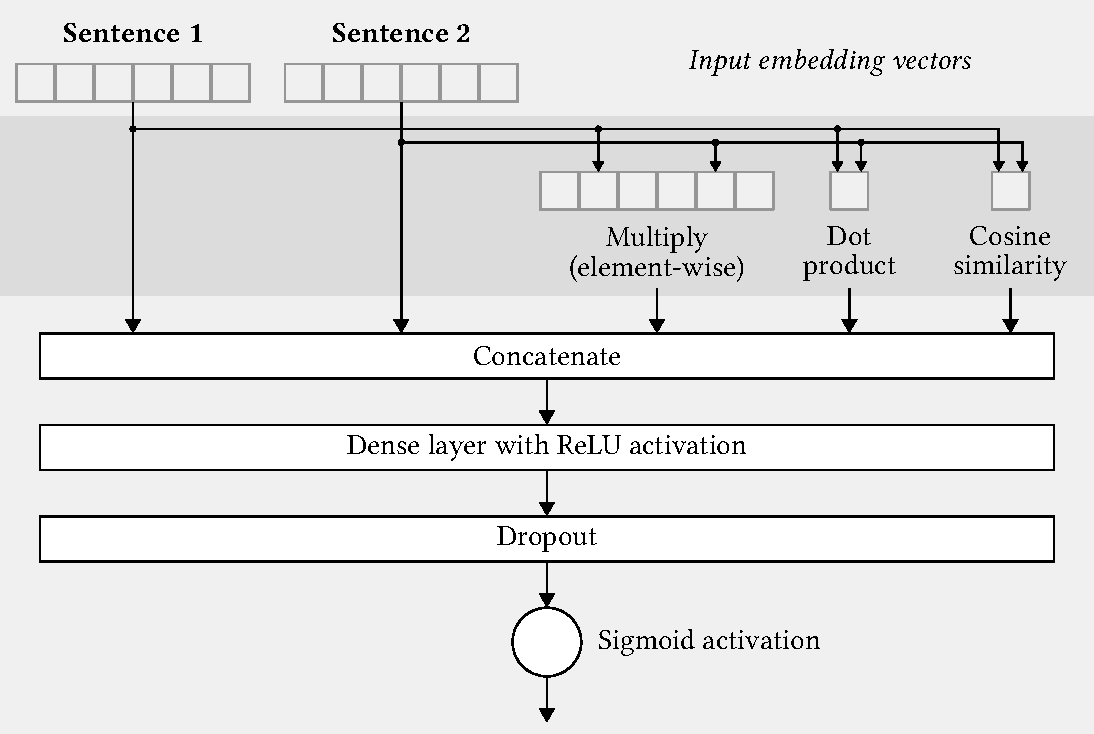
\includegraphics[width=\linewidth]{img/2019-n2c2-nn/v6/img.pdf}
\caption%
[Neural network architecture using sentence embeddings for measuring semantic textual similarity.]%
{Neural network architecture using sentence embeddings for measuring semantic textual similarity. ReLU: rectified linear unit.}
\label{fig:2019-n2c2-nn}
\end{figure}


For fine-tuning the hyperparameters and adapting the model architecture we used repeated K-fold cross-validation where for each repetition we applied cross-validation with the training data being split into three subsets: training, validation, and test.
These allowed for consistent model development without biasing in regard to the test set.
We used the training subset to update the network weights, the validation subset to evaluate the model performance in each epoch, and finally the test subset was used for unbiased evaluation.
The model that obtained the highest result in the validation subset was chosen to evaluate model performance in the test subset.
Model training was halted when the performance in the validation subset did not improve for a period of~20~epochs.

After this intensive model refinement with thorough evaluation on training data, the configuration model was left unmodified to be applied on unseen test data.
In the next section we evaluate the impact of using different pre-processing approaches, as well as using word embeddings or sentence embeddings as input vectors in the proposed neural network model.


\subsection{Results and discussion}

For gathering results we applied different text pre-processing pipelines and sentence representations: word embeddings \versus\ sentence embeddings.
We evaluated performance on (1) training data using repeated cross-validation and on (2) test data from predictions of a single evaluation.
Results presented in the training set were obtained by averaging~30 separate scores, whereas evaluation on test data was slightly different: we averaged the predictions of~30 individual models.
The idea behind this was to increase model robustness against the test data, because the final model is able to `see', and learn from, the whole training data by using diverse folds for training and validation.

During model development on training data, a compromise between the sizes of training, validation, and test subsets sizes was necessary.
Because of that, we explored the use of different K-fold split values to assess the impact of using less data for training and more for validation, and \viceversa.
We hypothesized that an optimal threshold considering enough training data and a solid evaluation on validation data could reflect an improvement on unseen data.

\begingroup

% \renewcommand{\arraystretch}{1.2}
\setlength\tabcolsep{4.0pt}

\begin{table}[!t]

\caption%
[Pearson correlation results obtained in the training and test sets of the 2019 \as{n2c2}/\as{ohnlp} Track~1 dataset.]%
{Pearson correlation results obtained in the training and test sets of the 2019 \as{n2c2}/\as{ohnlp} Track~1 dataset by averaging, respectively, the results and the predictions of 30 individual models (number of folds~$\times$~number of repetitions). For each distinct K-fold evaluation, the results of the configuration that obtained the highest performance in the training set, together with the corresponding results in the test set, are highlighted in bold. WE: word embeddings normalized sum. SE: sentence embeddings.}
% F: number of folds. R: number of repetitions.
\label{tab:2019-n2c2-results}

\centering

\small
% \footnotesize
% \scriptsize
% \tiny

\begin{tabular}{lllT{25mm}T{25mm}T{25mm}}

\toprule

Set & Features & Text pre-processing & 10-fold & 5-fold & 3-fold\\
& & & (3 repetitions) & (6 repetitions) & (10 repetitions)\\

\midrule
% \cmidrule{1-1}\cmidrule{2-2}\cmidrule{3-3}\cmidrule{4-6}

Training & WE & Base    & 0.716 & 0.735 & 0.672\\
         &    & Full    & 0.795 & 0.794 & 0.770\\
         &    & Partial & 0.771 & 0.773 & 0.728\\

\cmidrule{2-6}
% \cmidrule{2-2}\cmidrule{3-3}\cmidrule{4-6}

& SE & Base    & \textbf{0.811} & 0.810          & \textbf{0.792}\\
&    & Full    & 0.750          & 0.771          & 0.692\\
&    & Partial & 0.809          & \textbf{0.812} & 0.791\\

\midrule
% \cmidrule{1-1}\cmidrule{2-2}\cmidrule{3-3}\cmidrule{4-6}

Test & WE & Base    & 0.804 & 0.786 & 0.802\\
     &    & Full    & 0.823 & 0.826 & 0.824\\
     &    & Partial & 0.819 & 0.818 & 0.819\\

\cmidrule{2-6}
% \cmidrule{2-2}\cmidrule{3-3}\cmidrule{4-6}

& SE & Base    & \textbf{0.837} & 0.831          & \textbf{0.836}\\
&    & Full    & 0.808          & 0.780          & 0.802\\
&    & Partial & 0.818          & \textbf{0.819} & 0.826\\

\bottomrule

\end{tabular}
\end{table}
\endgroup


\Cref{tab:2019-n2c2-results} presents detailed results from all these experiments.
In general, the use of sentence embeddings provided superior results especially when using the base text pre-processing.
Surprisingly, the full text pre-processing provided better results when using word embeddings, proving the benefit of stop words removal.
To assess the effect of using different K-fold splits, we highlight the top scores according to the evaluation in the training set: for 10, 5, and 3-folds these were, respectively, 0.811, 0.812, and 0.792 in training data, and 0.837, 0.819, and 0.836 in test data.
Therefore, we conclude that the use of different splits for training and validation did not affect significantly the results, and thus any of the number of folds we used would be acceptable.

The highest scoring model in training data (0.812), which consisted in using sentence embeddings with partial text pre-processing (5-fold setting), produced a correlation of 0.819 in test data.
However, better results on test data were achieved when using sentence embeddings with the base text pre-processing (0.837, 0.831, and 0.836 for 10, 5, and 3-folds respectively).
Furthermore, it is interesting to notice that word embeddings with full text pre-processing also attained good test results (0.823, 0.826, and 0.824 for 10, 5, and 3-folds respectively) similarly to those with sentence embeddings.
Based on this, we believe that a careful combination of word and sentence embeddings may provide further improvement.

Overall, when analyzing training and test performances it is noteworthy that systems obtained higher scores on test data by a margin of approximately~0.02.
We suspect that one of the reasons for this is the fact that evaluation on test data was performed by averaging several models (where each model was trained and validated on distinct data subsets) whilst the results reported on training data are the average of several simulations made by an individual model.

Finally, we compare our highest test result (0.837) with those achieved during the 2019 \as{n2c2}/\as{ohnlp} clinical \as{sts} task \parencite{wang2020d} where a total of 87~valid system predictions were submitted: final aggregated results (Pearson correlation) presented a mean correlation of~0.712, a median of~0.829, and a maximum of~0.901.
We consider that our model attained a positive performance given its simplicity, being slightly above the median score, but also that there still exists large margin for progress given the maximum result achieved.


\subsubsection{Error analysis}

\begingroup

% \renewcommand{\arraystretch}{1.2}
\setlength{\tabcolsep}{6.4pt}

\begin{table}[!t]

\caption%
[Error analysis of predictions on the 2019 \as{n2c2}/\as{ohnlp} Track~1 dataset.]%
{Error analysis of predictions on the 2019 \as{n2c2}/\as{ohnlp} Track~1 dataset. Performance evaluation for different similarity levels using the following model from \Cref{tab:2019-n2c2-results}: sentence embeddings, base text pre-processing, and 10-fold evaluation. The three highest F1-scores in each set are highlighted in bold.}
\label{tab:2019-n2c2-analysis}

\centering

\small
% \footnotesize
% \scriptsize
% \tiny

\begin{tabular}{lcccccccccc}

\toprule

Metric & \multicolumn{5}{l}{Training} & \multicolumn{5}{l}{Test}\\

\cmidrule(r){1-1}\cmidrule(lr){2-6}\cmidrule(l){7-11}

& [0, 1] & ]1, 2] & ]2, 3] & ]3, 4] & ]4, 5] & [0, 1] & ]1, 2] & ]2, 3] & ]3, 4] & ]4, 5]\\

Precision & 0.826 & 0.206 & 0.361 & 0.488 & 0.491 & 0.853 & 0.115 & 0.097 & 0.365 & 0.318\\
Recall    & 0.416 & 0.362 & 0.244 & 0.625 & 0.532 & 0.269 & 0.391 & 0.188 & 0.307 & 0.618\\

F1-score  & \textbf{0.553} & 0.263 & 0.291 & \textbf{0.548} & \textbf{0.511} & \textbf{0.409} & 0.177 & 0.128 & \textbf{0.333} & \textbf{0.420}\\

\bottomrule

\end{tabular}
\end{table}
\endgroup

% Training - SE - Base - 0.811
%
%     MODE 2 evaluation [same interval]
%     --------------------------------------  --------------
%     [0, 1]  ]1, 2]  ]2, 3]  ]3, 4]  ]4, 5]   Micro-average
% ------------------------------------------  --------------
% TP     389     167     288     954     435            2233
% FP      82     644     510    1000     451            2687
% FN     546     294     892     572     383            2687
% P   0.8259  0.2059  0.3609  0.4882  0.4910          0.4539
% R   0.4160  0.3623  0.2441  0.6252  0.5318          0.4539
% F1  0.5533  0.2626  0.2912  0.5483  0.5106          0.4539
% ------------------------------------------  --------------

% Test - SE - Base - 0.837
%
%     MODE 2 evaluation [same interval]
%     --------------------------------------  --------------
%     [0, 1]  ]1, 2]  ]2, 3]  ]3, 4]  ]4, 5]   Micro-average
% ------------------------------------------  --------------
% TP      64      18       6      19      21             128
% FP      11     139      56      33      45             284
% FN     174      28      26      43      13             284
% P   0.8533  0.1146  0.0968  0.3654  0.3182          0.3107
% R   0.2689  0.3913  0.1875  0.3065  0.6176          0.3107
% F1  0.4089  0.1773  0.1277  0.3333  0.4200          0.3107
% ------------------------------------------  --------------


A detailed error analysis was performed to better understand model behaviour---that is, which similarity levels the model predicted more correctly---and to perceive if this could be another reason that made results on the test set higher than those on the training set (due to the dataset imbalance).
As such, we used the same similarity intervals as expressed in the dataset statistics (\Cref{tab:2019-n2c2-dataset}): [0,~1], ..., ]4,~5].

To perform this evaluation, we started by computing the number of true positives, false positives, and false negatives to calculate precision, recall, and F1-score.
A prediction was considered a true positive if the ground-truth was in the same similarity interval.
Otherwise, the prediction was assigned as false positive and false negative in the corresponding intervals.
To demonstrate this procedure, assume the model prediction is 3.7 whereas the ground-truth is 4.1.
In such case, a false positive and a false negative would be added in the similarity intervals ]3,~4] and ]4,~5], respectively.

\Cref{tab:2019-n2c2-analysis} presents this detailed error analysis in training and test data for a model with the following configuration: sentence embeddings, base text pre-processing pipeline, and 10-fold evaluation.
Overall, it is noticeable that the system had more difficulty in correctly predicting sentence pairs with scores in the interval ]1,~3].

It is interesting to note that the highest precision (around 0.8) was observed in the interval [0,~1] showing the model's ability to correctly detect completely dissimilar sentences.
Since the majority of samples (around 58\%) in test data were in this interval, this also supports our assumption that test results were higher because of their scores imbalance.
Additionally, one can observe that F1-scores were higher in extreme similarity intervals, corroborating the assumption from \textcite{wang2018e} that machines can succeed at distinguishing completely similar or dissimilar sentence pairs but, alike humans, they struggle in distinguishing less clear relations of semantic similarity.

Finally, despite the fact that F1-scores on test data are somewhat smaller to those on training, we emphasize this type of error analysis does not elucidate directly the model performance, since (1) the test set is highly imbalanced and (2) near-correct scores can be misinterpreted as complete failures as they fall in a different interval by a slight margin (for example the model predicts a score of 0.9 whereas the ground-truth is 1.1).


\section{Summary}

In this chapter we presented methods for text classification and semantic textual similarity measurement.
Regarding text classification, we described two different systems: one for identifying biomedical scientific abstracts that describe genetic mutations affecting protein--protein interactions; and a second one to classify certain criteria according to patients' clinical records.
For text similarity measurement we proposed a system that calculates the semantic agreement between clinical sentences.

We obtained competitive results with deep learning models in text classification when there was enough training data.
However, in the case of classifying clinical narratives the dataset was relatively small and our results with deep learning were significantly lower which emphasizes the need of having sufficient labeled data.
In that case, we had to create handcrafted rules or use traditional machine learning.
For text similarity measurement, deep learning performed relatively well with the use of word embeddings or sentence embeddings.

Text classification and measurement of semantic textual similarity were studied in this same chapter since it is our understanding that these tasks partly overlap.
For instance, documents with disparate semantic similarity may correspond to different topics in a text classification task.
However, we also recognize that text similarity measurement has use beyond text classification and can be applied in other tasks such as sense disambiguation in which contexts of ambiguous terms are compared.

We stress that pre-selecting appropriate documents for mining a particular type of biomedical knowledge is a crucial step oftentimes performed manually by domain experts and that text classification algorithms may assist, or even surpass, human annotation requiring reduced manual effort.
Thereby, techniques for improving biomedical text classification must continue to be investigated.
